\documentclass[12pt]{ucthesis}

\usepackage{array, floatrow, tabularx, makecell, booktabs, outlines}
\usepackage{multirow}  % span text across multiple rows
\usepackage{rotating}  % to write text vertically in a cell

\usepackage{etex}
\usepackage[morefloats=125]{morefloats}
\usepackage[hyphens]{url}
\usepackage[caption=false]{subfig}
\usepackage{graphicx}
\usepackage{tabularx}
\usepackage{amssymb}
\usepackage{amsmath}
\usepackage[letterpaper]{geometry}
\usepackage[overload]{textcase}
\usepackage{color}
\usepackage[nonumberlist,toc]{glossaries}
\usepackage{wrapfig}
\usepackage{longtable}
\usepackage{morefloats}
\usepackage{float}
\usepackage{listings}
\usepackage{makecell}
\usepackage{appendix}
\usepackage[]{algorithm2e}
\usepackage{titlesec}
\usepackage[breaklinks=true,hidelinks,pdfusetitle]{hyperref}
\usepackage{cleveref}
\usepackage{ifthen}

\setcounter{secnumdepth}{3}
\setcounter{tocdepth}{3}

% Added to avoid windows and orphans
\usepackage[all]{nowidow}
% Added to fix spacing between footnote entries
\usepackage{setspace}
\newlength{\myfootnotesep}
\setlength{\myfootnotesep}{\baselineskip}
\addtolength{\myfootnotesep}{-\footnotesep}
\setlength{\footnotesep}{\myfootnotesep} % set spacing between footnotes

\makeindex
\makeglossaries

% Shrink the size of headers
\titleformat{\chapter}[display]
        {\normalfont\normalsize\centering}
        {\ifthenelse{\equal{\thechapter}{A}}{APPENDICES\\[4.3ex]}{}\chaptertitlename\ \thechapter}
        {0pt}{\normalsize\uppercase}
\titlespacing*{\chapter}{0pt}{-20pt}{4.3ex plus .2ex}


\titleformat*{\section}{\normalsize\bfseries}
\titleformat*{\subsection}{\small\bfseries}
\titleformat*{\subsubsection}{\small\bfseries}
\titleformat*{\paragraph}{\small\bfseries}
\titleformat*{\subparagraph}{\small\bfseries}

\bibliographystyle{abbrv}

% Make \tindent indent pages if you have no paragraph indent
\newlength\tindent
\setlength{\tindent}{\parindent}
\setlength{\parindent}{0.in} \setlength{\parskip}{1.em}
\renewcommand{\indent}{\hspace*{\tindent}}
% Otherwise, comment out the above and uncomment this for default indentation on each paragraph
%\setlength{\parindent}{0.25in} \setlength{\parskip}{6pt}

\geometry{verbose,nohead,tmargin=1in,bmargin=1in,lmargin=1.5in,rmargin=1in}

% Different font in captions (single-spaced, bold) ------------
\newcommand{\captionfonts}{\small\bf\ssp}

\newcommand{\mycaption}[2]{\caption[#1 --- #2]{#1 --- #2}}

\makeatletter  % Allow the use of @ in command names
\long\def\@makecaption#1#2{%
  \vskip\abovecaptionskip
  \sbox\@tempboxa{{\captionfonts #1: #2}}%
  \ifdim \wd\@tempboxa >\hsize
    {\captionfonts #1: #2\par}
  \else
    \hbox to\hsize{\hfil\box\@tempboxa\hfil}%
  \fi
  \vskip\belowcaptionskip}
\makeatother   % Cancel the effect of \makeatletter
% ---------------------------------------

% Define Appendix refs
\crefname{app}{appendix}{appendices}
\Crefname{app}{Appendix}{Appendices}

% Add Figures folder to the graphics path
\graphicspath{{Figures/}{figures/}}

% Options for hyperref
\hypersetup{
    bookmarksnumbered=true,
    bookmarksopen=false,
    bookmarksopenlevel=0,
    colorlinks=false,
    pdfstartview=Fit,
    pdfborder={0 0 0},
}

\newcounter{qcounter}
\providecommand{\keywords}[1]{\textbf{\textit{Keywords:}} #1}


\newcommand{\titletext}{Adapting Single-View View Synthesis with Multiplane Images for 3D Video Chat}


\begin{document}

% Declarations for Front Matter
% \title{Bringing a 3D Effect to Video Chats by Synthesizing Novel Views via Multiplane Images}
% \title{Video Chat View Synthesis using/with Multiplane Images}
% \title{Adapting Single-View View Synthesis using/with Multiplane Images to Video Chat Scenarios}
% \title{Dataset Experiments for Learning Single-View View Synthesis using/with Multiplane Images in Video Chat Scenarios}

% Refer new command \titletext in main.tex
\title{\titletext{}}

\author{Anurag Uppuluri}
\degreemonth{December} \degreeyear{2021} \degree{Master of Science}
\defensemonth{December} \defenseyear{2021}
\numberofmembers{3}
   \chair{Jonathan Ventura, Ph.D. \linebreak Assistant Professor of Computer Science}
   \othermemberA{Zo\"{e} Wood, Ph.D. \linebreak Professor of Computer Science}
   \othermemberB{Franz Kurfess, Ph.D. \linebreak Professor of Computer Science}
\field{Computer Science} \campus{San Luis Obispo}
\copyrightyears{seven}


\maketitle

\begin{frontmatter}

% Custom made for Cal Poly (by Mark Barry, modified by Andrew Tsui).
\copyrightpage

% Custom made for Cal Poly (by Andrew Tsui).
\committeemembershippage

\begin{abstract}
Activities like one-on-one video chatting and video conferencing with multiple participants are more prevalent than ever today as we continue to tackle the pandemic. Bringing a 3D feel to video chat has always been a hot topic in Vision and Graphics communities. In this thesis, we have employed novel view synthesis in attempting to turn one-on-one video chatting into 3D. We have tuned the learning pipeline of Tucker and Snavely's~\cite{single_view_mpi} single-view view synthesis paper --- by retraining it on \textit{MannequinChallenge Dataset~\cite{li2019learning}} --- to better predict a layered representation of the scene viewed by either video chat participant at any given time. This intermediate representation of the local light field --- called a Multiplane Image (MPI) --- may then be used to rerender the scene at an arbitrary viewpoint which, in our case, would match with the head pose of the watcher in the opposite, concurrent video frame. We discuss that our pipeline, when implemented in real-time, would allow both video chat participants to unravel occluded scene content and ``peer into" each other's dynamic video scenes to a certain extent. It would enable full parallax up to the baselines of small head rotations and/or translations. It would be similar to a VR headset's ability to determine the position and orientation of the wearer's head in 3D space and render any scene in alignment with this estimated head pose. We have attempted to improve the performance of the retrained model by extending MannequinChallenge with the much larger \textit{RealEstate10K Dataset~\cite{zhou2018stereo}}. We present a quantitative and qualitative comparison of the model variants and describe our impactful dataset curation process among other aspects.
\end{abstract}

\begin{acknowledgements}
\noindent
Thanks to:
\begin{itemize}
    \item My advisor, Dr. Ventura, and all the other faculty and staff members here at Cal Poly I am fortunate to interact with, faculty and staff at Fresno State, Sathyabama University, and all the other schools I am an alumnus of, my family, and my friends for going above and beyond in helping me set sail in and even course through uncharted potential with oft-increasing frequency. It's as they say: you tend to a sapling until it takes firm root and starts bearing fruit. I feel all these people have been doing all that and more all along, and I can't wait to give back in ways that far surpass my imagination.
    \item Richard Tucker, for his selfless and infectious enthusiasm in guiding our project.
    \item Robert Downey Jr. as Tony Stark in Iron Man (2008) saying, ``Jarvis, sometimes you gotta run before you can walk," before pushing the limits of the Mark II armor.
    \item A Panda Express fortune cookie fortune for prophesizing ``Love first --- then everything will follow."
    \item Andrew Guenther, for uploading this template.
\end{itemize}

\end{acknowledgements}

\tableofcontents

% \listoftables

\listoffigures

% Add CHAPTER into table of contents.
\addtocontents{toc}{%
   \noindent CHAPTER
}

\end{frontmatter}

\pagestyle{plain}

\renewcommand{\baselinestretch}{1.66}

\chapter{Introduction}\label{ch1:introduction}
 
From pertinent work meetings to casual conversations with family and friends, an ever-increasing number of people use video chatting/conferencing applications such as FaceTime, Zoom, Google Meet, and Microsoft Teams, to name a few. One way of improving video chat experience is to bring in a feel of 3D by providing alternate views of each viewed scene, rendered at different viewpoints. To fortify the 3D experience, each novel view would have to be rendered at the right angle such that it aligns with the viewpoint of the viewer. This would require taking the viewer's transient head pose\footnote{Pose refers to the combination of any object's (including a camera's) position and orientation in 3D world space. In contrast, we only use the \textit{orientation} of the viewer's head in the world as the head pose for viewed scenes to be rerendered at.} into account. In this way, we can seek to get an ideal feel of 3D by, essentially, simulating what happens when we move our heads. Whenever we move our heads, what we see in terms of the extent of the foreground, the background, and everything in between changes based on our changing head poses. These changes need to be reflected in rendered novel views. In this work, we attempt to emulate 3D video chatting via targeted, high-quality novel view synthesis.

\section{Motivation}\label{sec:motivation} 

\begin{figure}[!h]
    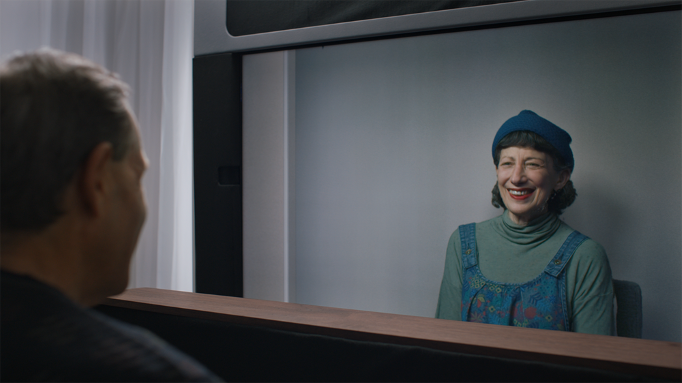
\includegraphics[width=1\columnwidth]{figures/google-starline-416.png}
    \caption{Google's Project Starline~\cite{}}
    \label{fig:google-starline}
    {\small Project Starline is reported to use a groundbreaking light field rendering system that will improve glasses-free 3D / automultiscopic video chat experience by leaps and bounds when it releases later this year.}
\end{figure}

Currently, synthesis of high-quality novel views --- the basis of Image-Based Rendering (IBR) systems --- is difficult to achieve end-to-end without some form of an intermediate representation of the structure (such as 3D world points) of the scene depicted by the given image(s). For instance, Google's Project Starline (Figure~\ref{fig:google-starline}) is reported to use a dense 3D representation to go from known views to novel views. One impressive variation of such an intermediate representation is called a Multiplane Image (MPI) --- first reintroduced in Zhou et al.~\cite{zhou2018stereo} (Figure~\ref{fig:mpi-layered-representation}). It is a volumetric representation that reprojects 2D points making up an image onto multiple 2D planes situated one behind the other at successive depths along the z-axis, according to the computed depth/disparity value(s)\footnote{Since pixels are generally smaller in size than points, there can be multiple RGBA and depth/disparity values corresponding to the multiple pixels that might make up a 2D point on an image.} at each point to be mapped. MPI planes are parallel to each other and also to a reference coordinate frame centered at a reference camera/viewpoint looking down positive z-axis. The reference camera can be that of the image itself or of a different view of the scene captured by the image. An MPI can thus be formulated as a set of RGBA layers $\{(C_1,\ \alpha_1),\ (C_2,\ \alpha_2),\ \ldots,\ (C_D,\ \alpha_D)\}$, where $C_i$ refers to the RGB map of each layer $(C_i,\ \alpha_i)$ and $\alpha_i$ is the alpha map. $D$ is the total number of depth planes used in the MPI. To render from an MPI one simply needs to alpha-blend all layers in back-to-front order, as explained in section~\ref{sec:learning-mpis}. One popular instance of such depth planes used in an MPI is a set of 32 planes positioned at equidistant disparity, with the near and far planes being at 1m and 100m in 3D world space, respectively. Since disparity is inversely proportional to depth, the points on the nearer MPI planes are closer to the reference camera than the ones on the farther planes but they have greater disparity values associated with them than the farther ones.

\begin{figure}[!h]
    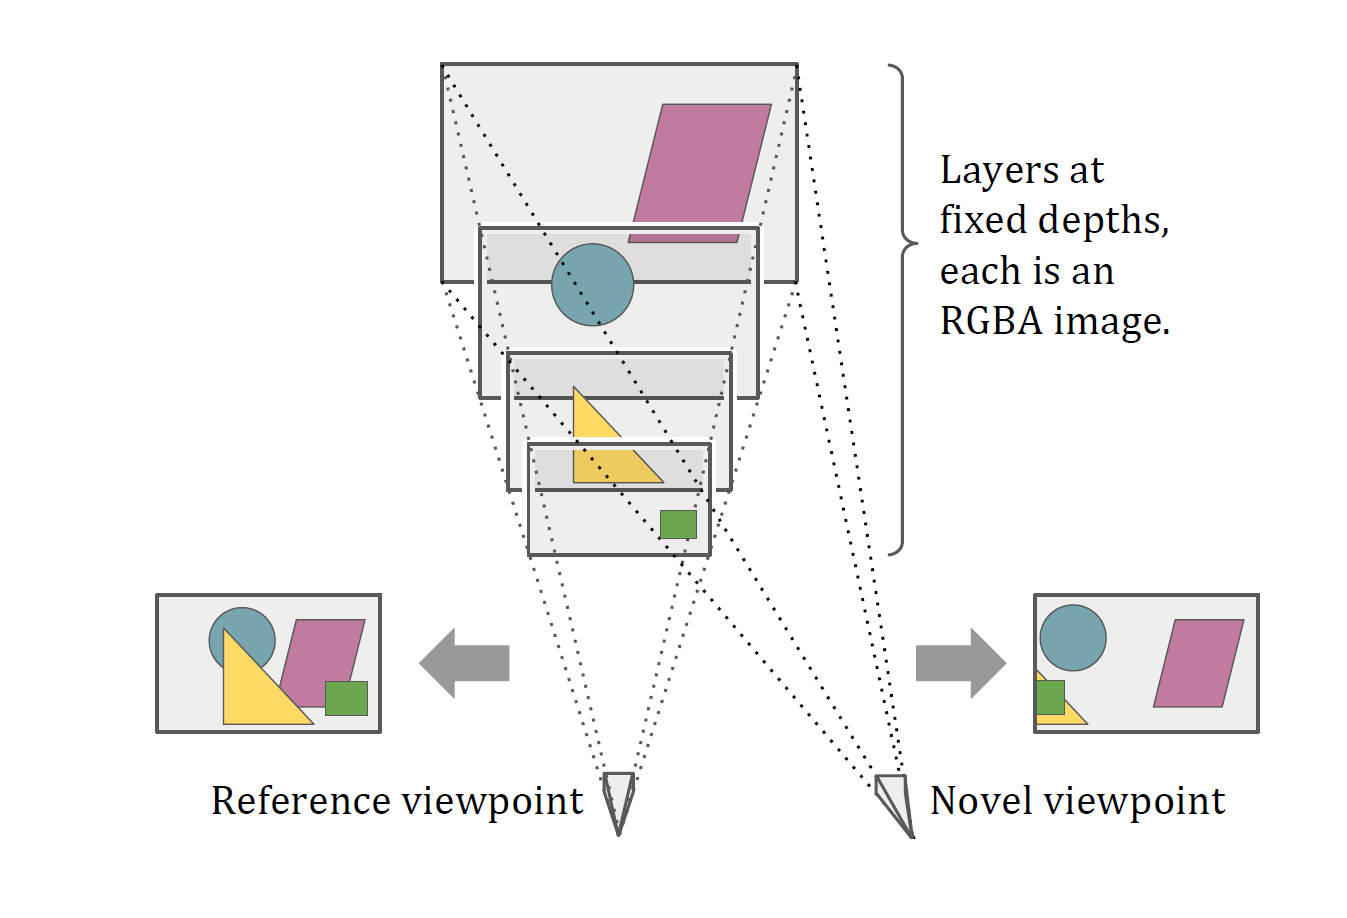
\includegraphics[width=1\columnwidth]{figures/mpi-layered-representation.png}
    \caption{The Volumetric/Layered MPI Representation}
    \label{fig:mpi-layered-representation}
    {\small A given image is reprojected onto multiple fronto-parallel MPI planes within the view frustum a common reference viewpoint that may or may not match with the given image's viewpoint. A novel image is synthesized by alpha-blending these intermediate layers in back-to-front order.}
\end{figure}

\begin{figure}[!h]
    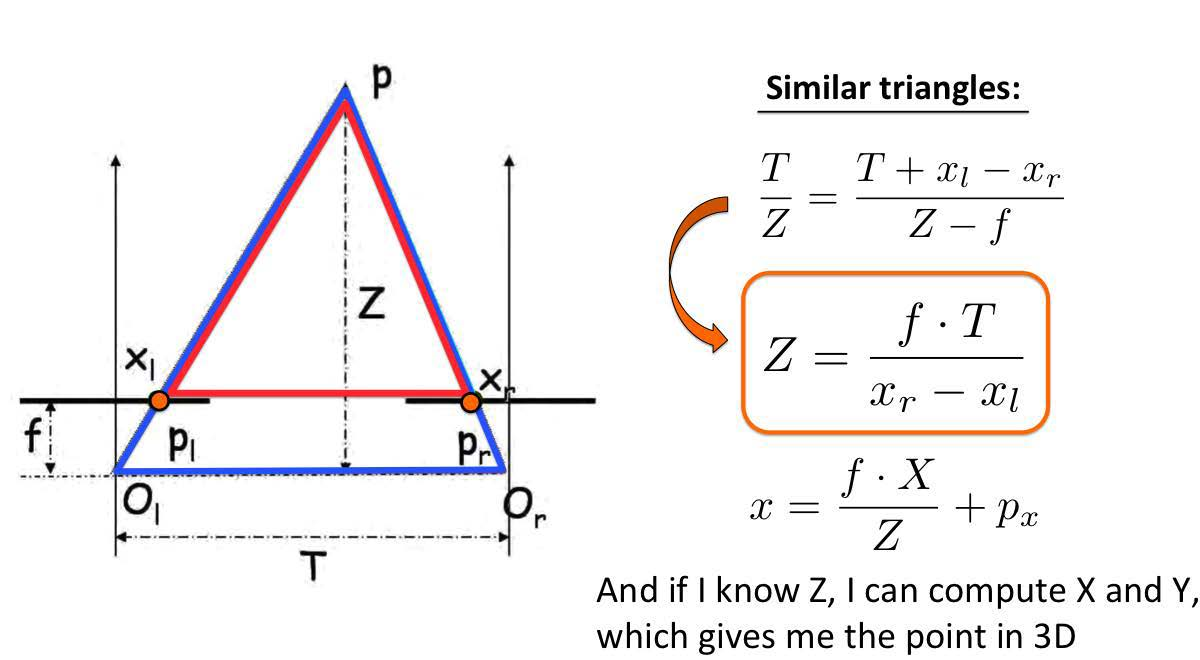
\includegraphics[width=1\columnwidth]{figures/disparity-triangulation.png}
    \caption{Disparity used in Triangulating 3D Points~\cite{fidler_depth_2021}}
    \label{fig:disparity-triangulation}
    {\small In this birds-eye view down the y-axis, $O_l$ and $O_r$ are the optical/camera centers of the left and right images of a stereo pair, $p_l$ and $p_r$ are the 2D projections of the same 3D world point $p$ onto the stereo pair, $x_l$ and $x_r$ are the x-coordinates of these 2D image points (y-coordinates are the same for corresponding points on a stereo pair), $f$ is the common focal length of the stereo cameras, $T$ is the horizontal translation or baseline of the stereo cameras, and $Z$ is the perpendicular depth of $p$ from the common reference coordinate frame of the stereo cameras and is inversely proportional to the disparity, $x_r - x_l$. Taking similar birds-eye perspectives down the $z$ and $x$ axes, we can compute the $x$ and $y$ coordinates of the 3D point as well.}
\end{figure}

Disparity refers the number of pixels that each point on a image shifts over by in any of its warped/transformed counterparts that can relate to it via a homography (projective transform function). Disparity is required for triangulating the depth(s) at each point on the image with respect to its warped version(s). Triangulating depth and estimating the 3D scene structure is easier when two or more of the scene's images are subjected to either stereo or multi-view image rectification, respectively. Such image rectification procedures typically involve rotating and shifting the optical centers of each image so they became collinear and scaling --- adjusting the focal lengths of the cameras of --- the images themselves so they become coplanar. Rectified image sets are characterized by point displacements only in the horizontal/row-wise $x$ direction. Properties of similar triangles can then be applied to the rectified images to get at the z-coordinate of each 3D world scene point most agreed upon by all the images containing the point's projections, after accounting for reprojection mismatches. Figure~\ref{fig:disparity-triangulation} shows the triangulation process for a stereo pair. This is akin to how the human visual system (including the eyes, the ganglia therein, the dorsal and ventral streams of the brain, and the visual cortex) is able to triangulate depth from binocular vision. The brain is backed by prior knowledge, heuristics, and biases (made apparent by optical illusions) that it is able to use to infer depth to some degree of approximation even with one eye closed. Since Artificial Neural Networks (ANNs) are basically trying to replicate and someday even surpass the workings of the human brain, we are actually trying to fill in for this prior knowledge acquired by the brain when we provide ANNs with copious amounts of data to learn from and devise their own heuristics out of. Therefore, we may only generate an MPI for an image when we are provided either with one or more shifted and/or rotated reprojections of the scene in the image or with the homographies for generating each of these transformed images from the original image. Otherwise, we would need to be supplied the sparse/dense 3D point cloud of the image's scene itself. 
\section{Contribution}\label{sec:contribution} 

To give a gist of our work, it began by attempting to retrain Tucker and Snavely's state-of-the-art end-to-end fully-convolutional single-view view synthesis with MPIs CNN~\cite{single_view_mpi} on the MannequinChallenge dataset. We hypothesized --- as was also hinted at in the paper --- that such retraining would be sufficient to generate high quality MPIs of scenes involving close-up shots of people, typical of video chat settings. The original model is able to do the same for real estate scenes. We then went on to compare the inference results of this primary model variant with those of another variant trained on the MannequinChallenge dataset extended by the RealEstate10K dataset, taking the pretrained Tucker and Snavely model as baseline. This was so we could determine the best variant to apply to the domain of 3D video chat. Such application was conceived to be by way of a two-way rendering of appropriate novel views of concurrent dynamic scenes viewed by one-on-one video chat participants in both directions simultaneously. In the two-way pipeline, a novel view of a video frame would be rendered every time a change in head pose is detected in the participant in the opposite frame. To our knowledge, MPIs have not been used in 3D video chat so far. We publish the code used to fill in the missing parts of Tucker and Snavely's publicly available training and testing pipelines, along with highlights regarding curating and taking advantage of both datasets for view synthesis in video chats.


\chapter{Related Work and Background}\label{ch2:related-work-background}

In this thesis, we have not created novel models or datasets but have curated preexisting datasets and retrained a state-of-the-art CNN. Data curation has been an essential part of our work as the datasets' YouTube videos are subject to modifications over time. These modifications are in terms of the videos being taken down from YouTube or the required 1280x720 pixel (720p) versions of them becoming unavailable, etc. The curation process included action items like downloading and using only 720p resolution videos across the board so as to minimize the chances of running into training errors, etc., as explained in section~\ref{sec2:data}. As for simulating the 3D video chat experience itself, we linked up the API of OpenFace 2.2 --- a preexisting head pose estimation model --- to the MPI inference procedure so the MPI inference may generate novel views rendered in the head pose evaluated by OpenFace 2.2, as explained in section~\ref{sec3:implementation}

This chapter explores related work in two areas: MPIs and 3D video chat, while providing clarifications on background concepts along the way. The research papers of particular interest to us as far as the MPI component of our work is concerned are 2018's Zhou et al.~\cite{zhou2018stereo} and 2020's Tucker and Snavely~\cite{single_view_mpi}. This is because we have attempted to adapt and apply Tucker and Snavely's work to the purposes of video chatting and their work draws directly from Zhou et al. We have also sought to differentiate 2016's~\cite{deep_stereo_2016} and~\cite{kalantari_2016} from Zhou et al. as it, in turn, is heavily inspired by them and as they would be integral to understanding the motivations of Zhou et al. As for progress in the field of 3D video chat, we have mentioned the yet to be released state-of-the-art 3D video chat system: Google's Project Starline.

\section{Learning MPIs}\label{sec:approach} 

Some of the major challenges of high-quality novel view synthesis include synthesizing pixels occluded in one or more of the provided views, disentangling and localizing pixels at/near the boundaries of foreground and background objects, localizing pixels at transparent, translucent, or reflective surfaces, etc. Moreover, whereas interpolating novel views at desired viewpoints lying in between the given views is easier to achieve compared to extrapolating significantly beyond the baselines (distances between camera centers) of input viewpoints, these challenges are going to be present in either case. So far, it has been found that learning view synthesis is the way to go for tackling all these challenges in one shot. Before the Machine Learning (ML) boom in Computer Vision (CV) circles in 2012, convolutional filters had to be handcrafted and carefully layered one on top of the other before input views could be subjected to them and various types of features could be extracted to render novel views. All the aforementioned view synthesis challenges had to be manually targeted by way of devising various combinations of filters for each complication. This meant a high proportion of artifacts induced in novel views would be left unresolved. Since 2012, prominently and to the delight of the CV community, the need to handcraft filters was obviated by ML models that learned to design all required convolutional filters on their own in their various layers. These self-learnt filters are defined by the constantly improving weights and biases in each neuron of the network layers and are mostly specific to the datasets they are trained on, with some degree of generalizability to other datasets. If trained well under effective hyperparamter tuning, learnt filters can evolve to surpass manual filters in redressing occlusion, transparency, reflection, and other image synthesis problems.

View synthesis lends itself to being a semi-well-posed to well-posed learning problem where two or more images of a scene can be shot and an ML model can be exposed to one of more of these images while being expected to predict one or more of the remaining views that have been withheld from it. The quantitative difference between the corresponding predicted and withheld (ground truth) views will then be the loss that the ML training seeks to minimize. Since, end-to-end view synthesis without an intermediate representation is still largely unrealized, the popular way to synthesize novel views is to learn an intermediate representation of the scene common to the input views and use this intermediate representation to render novel views. The MPI intermediate representation has proven to be one the most effective representations for this purpose with implications as significant as real-time high-quality view synthesis. The roots of the MPI representation may be traced back to seminal work such as 1996's \cite{collins_space-sweep_1996} 1998's \cite{fft} and 1999's \cite{fft} --- the 1996, 1998, and 1999 papers. The 1996 paper first perfected the concept of plane sweep volumes, the 1998 paper introcuded layered depth images and the 1999 paper the actual MPI representation itself.
come back to come bcak and drive up thse gat eto come back and take down and take irt back up to the coming month and taeke it up bring it back to get it doen to coming permanent solutij andf come back and benglwts xoemhvfanadI thij I know hwo to ome abck anmd so they come down to the bring  and bring back dow to this situastio sand come back up to this case and down to this awesome ness and ope fuk ytsoend this timwe and lau dow to coming back to thisd lllcolbalt colamp did nothid but bundle adjustment sndf alignke and I wouf like to tske a lok at tho and 

Kalantari interpolates (fills in) novel views in the 8x8 (u,v) view grid of a lytro camera this grid is that of microlens arrays that has microlensing arrays 
The model the 

MPI scene representation is similar to Layered Depth Image (LDI) scene representation introduced by \cite{layered_depth_images}. Both MPI and LDI consist of a series of fronto-parallel planes facing the reference camera of one of the given images and placed at different depths from it. These planes contain the RGB information of the original pixels of the image(s), segregated according to depth. The difference between LDI and MPI is that MPI has alpha masking effects at each layer as it is generated with alpha transparency maps for each layer. Also, MPI has fixed depths for each layer as opposed to the varying layer depths of LDI.

MPI scene representation is similar to Layered Depth Image (LDI) scene representation introduced by \cite{layered_depth_images}. Both MPI and LDI consist of a series of fronto-parallel planes facing the reference camera of one of the given images and placed at different depths from it. These planes contain the RGB information of the original pixels of the image(s), segregated according to depth. The difference between LDI and MPI is that MPI has alpha masking effects at each layer as it is generated with alpha transparency maps for each layer. Also, MPI has fixed depths for each layer as opposed to the varying layer depths of LDI. 

\begin{figure}[!h]
    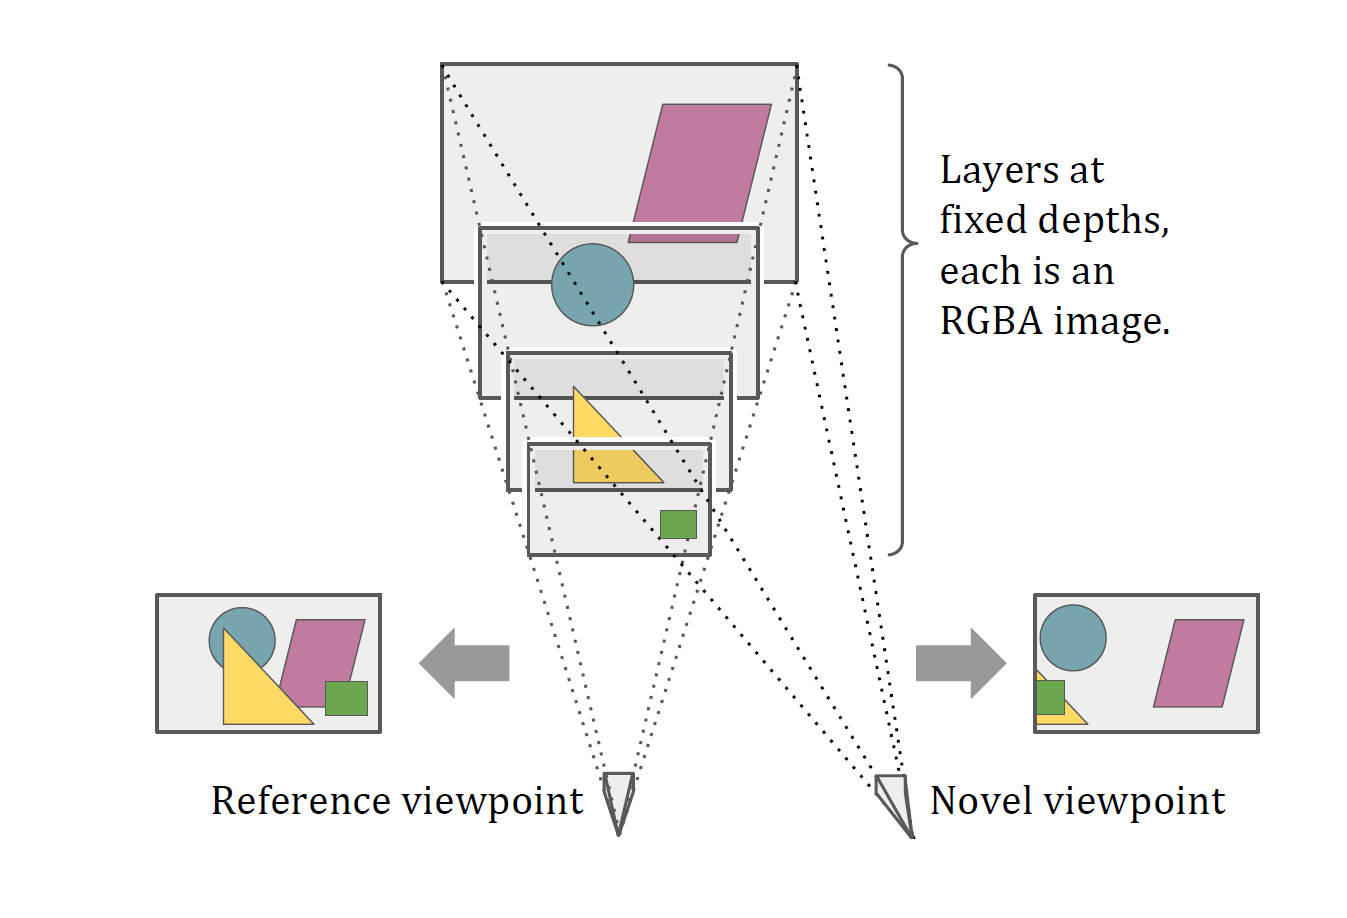
\includegraphics[width=1\columnwidth]{figures/mpi-layered-representation.png}
    \caption{Fronto-parallel planes in MPI layered representation}
    \label{fig:mpi-layered-representation}
\end{figure}
Fig 3. Example of fronto-parallel planes

The 2018's Stereo MPI and 2020's Single-View MPI papers have the similar training procedures of suppressing some frames from a video clip as ground truth, attempting to predict these frames and finally minimizing various loss metrics between the rendered frame and the suppressed frame.

\subsection{The 1999 paper}\label{subsec2:1999}
\subsubsection{The 1999 paper}\label{subsubsec2:1999}

The 1999 MPI paper first introduced the MPI representation for purposes of stereo matching, otherwise called disparity mapping. In this paper the authors used MPIs for matte separation of foreground and background in which they sample the 3D Cartesian space into a disparity space where a 3D point [x y z] would map to [x y 1 d]. Since disparity maps are a byproduct of the 2020 MPI model, it behoves us to explain here what they are. Disparity is nothing by the pixel distance between any two corresponding/matching pixels in stereo image pair. This correspondence or finding if the pixel occurs in both images of the stereo pair the can be determined by first running feature detection algorithms like SIFT and then subjugating the extracted features to realignment and finally to these depth prediction algorithms.

Stereo Matching is one of the core technologies in computer vision, which recovers 3D structures of real world from 2D images. It has been widely used in areas such as autonomous driving, augmented reality and robotics navigation. Given a pair of rectified stereo images, the goal of Stereo Matching is to compute the disparity for each pixel in the reference image, where disparity is defined as the horizontal displacement between a pair of corresponding pixels in the left and right images.
    
\begin{figure}[!h]
    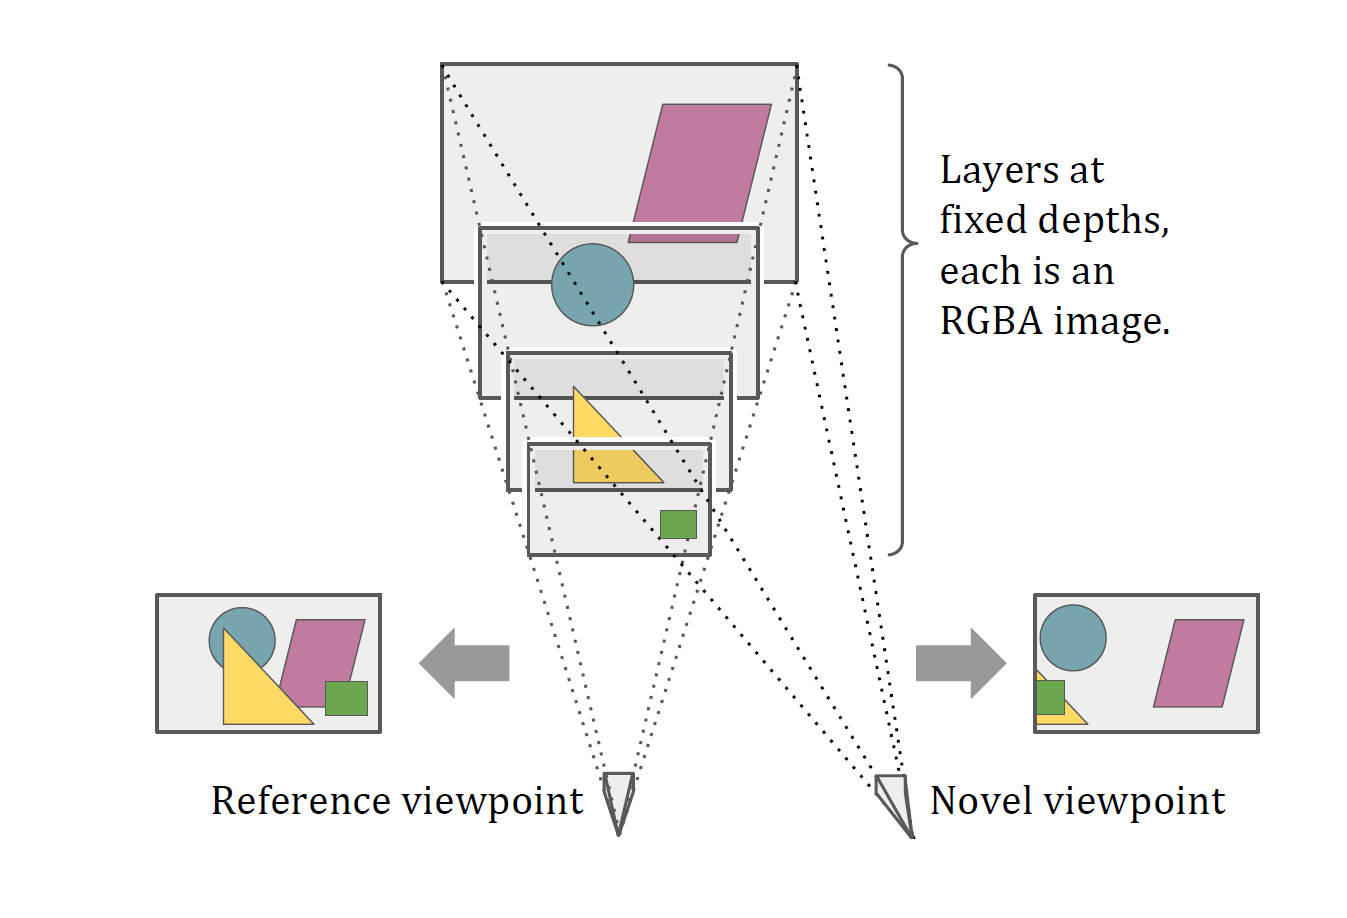
\includegraphics[width=1\columnwidth]{figures/mpi-layered-representation.png}
    \caption{Fronto-parallel planes in MPI layered representation}
    \label{fig:mpi-layered-representation}
\end{figure}
Fig 3. Example of fronto-parallel planes

To examine the novel stereo correspondence algorithm's features, the authors conducted a modest set of experiments on certain synthetic stereo datasets, evaluating both the algorithm's basic behavior and its performance on mixed pixels. Visualizing opacities/transparencies is critical for comprehending and validating the algorithm. As a result, the writers selected color stimuli. The authors began by creating a typical random-dot stereogram with k = 5 pictures, in which the camera geometry and filled disparity planes result in integral pixel shifts. This sample contains no pixels that are partially translucent. The first eight columns indicate the estimated colors and opacities of the eight disparity planes in (x, y, d) space.

While preliminary experimental results are intriguing, recovering correct depth, color, and opacity estimations simultaneously remains a difficult task. On the other hand, is to recover a poorly populated color and opacity volume. This has the advantage of accurately modeling mixed pixels and occlusion effects, allowing them to integrate photos taken from extremely dissimilar angles of view. It significantly complicates the estimation problem, as the number of free parameters frequently exceeds the number of data, necessitating the use of smoothness constraints and other previous models. To address these issues, it may be necessary to improve imaging and sensor models, or to work on a higher resolution picture grid.

The authors have created a novel framework for recovering disparities, hues, and opacities from several images concurrently. This framework enables them to cope with a variety of stereo matching issues that arise frequently, such as partially occluded regions and pixels that contain foreground and background color combinations. It promises to give higher-quality color and opacity estimations that can be used to extract foreground objects and blend real and synthetic imagery. This format can enable a far broader range of synthetic views than a single texture-mapped depth picture can in view interpolation applications.

 \subsection{The 2016 paper}\label{subsec2:2016}

Estimating 3D shape from multiple posed images is a fundamental task in computer vision and graphics, both as an aid to image understanding and as a way to generate 3D representations of scenes that can be rendered and edited. The authors aim to solve the related problem of new view synthesis, a form of image-based rendering (IBR) where the goal is to synthesize a new view of a scene by warping and combining images from nearby posed images. This can be used for applications such as cinematography, virtual reality, teleconferencing [4], image stabilization [19], or 3-dimensionalizing monocular film footage. Good approaches to IBR typically require the use of strong priors to fill in pixels where the geometry is uncertain, or when the target color is unknown due to occlusions The authors aim to solve the related problem of new view synthesis, a form of image-based rendering (IBR) where the goal is to synthesize a new view of a scene by warping and combining images from nearby posed images.
The authors' goal is to learn a model for predicting new viewpoints by directly minimizing the prediction error on the training set

To evaluate the model on view interpolation, the authors generated a novel image from the same viewpoint as a known image captured by the Street View camera.
The imagery from this prior work is quite different from the training images, as these prior images were taken with a handheld DSLR camera. Despite the fact that the model was not trained directly for this task, it did a reasonable job at reproducing the input imagery and at interpolating between them. These images were rendered in small patches, as rendering an entire image would be prohibitively expensive in RAM. The authors' current implementation does not fully exploit the convolutional nature of the model, so these times could likely be reduced to minutes or even seconds by a GPU implementation in the spirit of Krizhevsky, et al [20]

\begin{figure}[!h]
    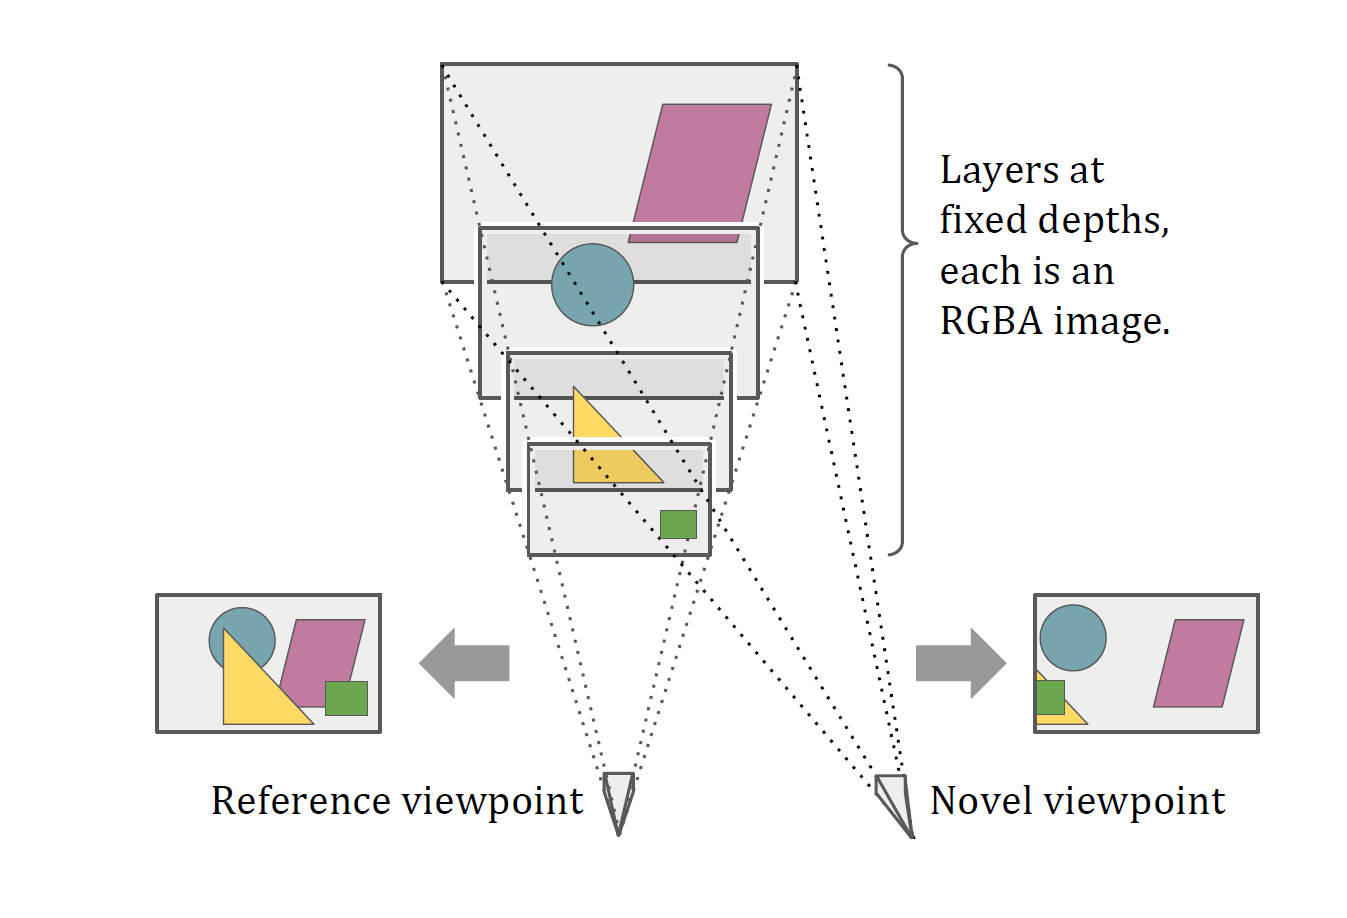
\includegraphics[width=1\columnwidth]{figures/mpi-layered-representation.png}
    \caption{Fronto-parallel planes in MPI layered representation}
    \label{fig:mpi-layered-representation}
\end{figure}
Fig 3. Example of fronto-parallel planes

The authors have shown that it is possible to train a deep network end-to-end to perform novel view synthesis. The authors' method currently requires reprojecting each input image to a set of depth planes; the authors currently use 96 depth planes, which limits the resolution of the output images that the authors can produce. Increasing the resolution would require a larger number of depth planes, which would mean that the network takes longer to train, uses more RAM and takes longer to run. This is a drawback shared with other volumetric stereo methods; the method requires reprojected images per rendered frame, rather than just once when creating the scene. The authors plan to explore pre-computing parts of the network and warping to new views before running the final layers

 \subsection{The 2018 paper}\label{subsec2:2018}

Motivated by the development of stereo cameras, this article investigates the difficulty of creating novel perspectives from such narrow-baseline image pairings. While most past work has focused on interpolating between a set of supplied views [Chen and Williams 1993], the authors concentrate on the problem of significantly extrapolating views beyond the two input images. This type of view extrapolation has a variety of uses in photography. The authors may seek to extend an IPD-separated stereo pair acquired with a VR180 camera to an entire set of views along a line, say half a meter in length, in order to achieve full parallax with a minimal range of head motion. The authors refer to this technique as stereo magnification, which involves extrapolating a view from a pair of input views. The authors require the ability to render pixels that are obscured and invisible in one of the input views. To overcome these issues, we will train our system to conduct view extrapolation from vast volumes of visual data, similar to recent work on view interpolation using deep learning [Flynn et al 2016; Kalantari et al 2016]. The authors seek a scene representation that can be predicted once given a pair of input views and then reused to predict a large number of output views, in contrast to past work that required prediction of each output view independently. The authors demonstrate that the learnt model generalizes to additional datasets without requiring retraining and is successful at amplifying the limited baseline of stereo vision acquired by cell phones and stereo cameras. Multiplane Images are a novel type of scene representation that can be used to do vision synthesis. A novel use of online video to the study of view synthesis, namely view extrapolation

\begin{figure}[!h]
    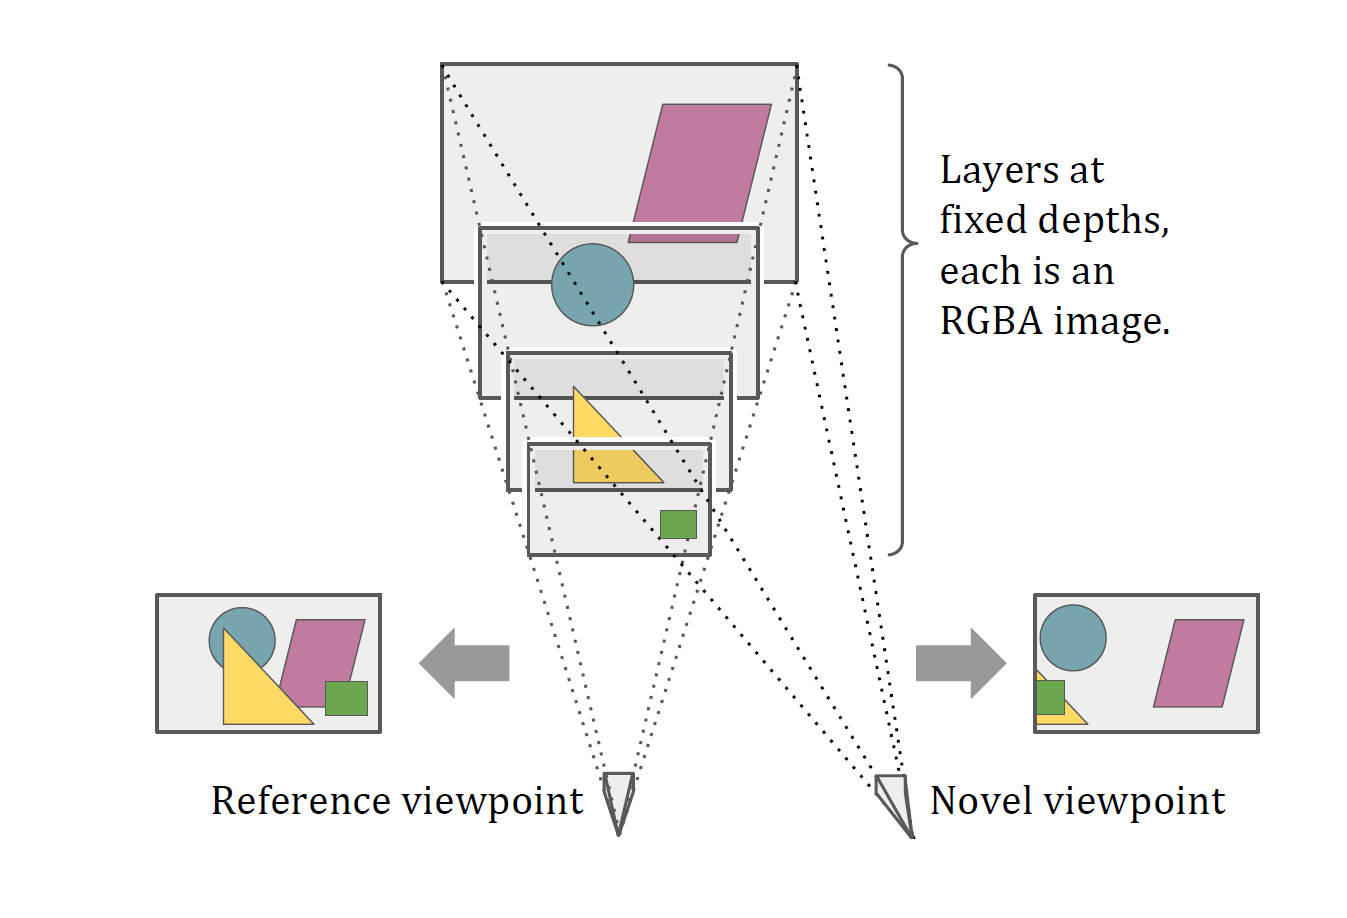
\includegraphics[width=1\columnwidth]{figures/mpi-layered-representation.png}
    \caption{Fronto-parallel planes in MPI layered representation}
    \label{fig:mpi-layered-representation}
\end{figure}
Fig 3. Example of fronto-parallel planes

An MPI is similar to the Layered Depth Image (LDI) representation proposed by Shade et al. [Shade et al 1998], except that the pixels in each layer are fixed at a specific depth, and the authors encode visibility using an alpha channel per layer. The authors' depiction is reminiscent of the multiplane camera pioneered at Walt Disney Studios and widely utilized in traditional animation. [2017, Wikipedia] A scene is made of a sequence of partially transparent layers at varying distances from the camera in both systems. Along with the input photos I1 and I2, the authors include their associated camera parameters. The predicted scene's reference coordinate frame is centered on the camera in the first input picture I1 (i.e., p1 is fixed to be the identity pose). The authors compute a plane sweep volume (PSV) that reprojects I2 into the reference camera at a set of D fixed depth planes in order to encode the pose information from the second input picture I2. The authors chose these depth planes to correspond to the output MPI's depth planes. The output of this plane sweep computation is a stack of reprojected pictures I1,. The network output might simply be a single RGBA image for each depth plane, with the color image capturing the scene's look and the alpha map encoding visibility and transparency. The authors assume that the scene's color information can be accurately modeled using only two images: a foreground and a background image, where the foreground image is the reference source I1 and the background image is predicted by the network and is intended to capture the appearance of hidden surfaces.

The network generates the following values: 1) an alpha map d for each plane, 2) a global RGB background image Ib, and 3) a blending weight image wd for each plane indicating the foreground and background layers' relative proportions at each pixel. If the authors forecast D depth layers with each layer having a resolution of W H, then the total number of output parameters is W H (2D + 3).
These values can be converted to an MPI value. The authors can generate a novel view using the MPI representation in relation to a reference frame. It accomplishes this by performing a planar transformation on the RGBA image for each plane, followed by an alpha-composition of the changed images into a single image in reverse order. Both the planar transformation and alpha composition are distinct operations that can be integrated into the remainder of the learning pipeline. The authors retrieve each pixel in the target MPI plane using typical inverse homography [Hartley and Zisserman 2003]. The authors can retrieve the color and alpha values for each target pixel [ut, vt ] by locating its correspondence in the source image [us, vs ]. The authors derive the expected target view by alpha compositing the color images in back-to-front order using the standard over operation after applying the planar transformation to each MPI plane [Porter and Duff 1984].

The authors can train a network to predict MPIs matching the view synthesis target given the MPI inference and rendering process. Although the pictures and MPI have a spatial resolution of 1024 576, the model may be fully convolutional applied to any resolution at test time. While many videos on YouTube are unsuitable for the purposes, the writers discovered a surprising amount of relevant content across a variety of video categories. Real estate footage is one such category. The typical real estate video consists of a succession of views of inside and exterior locations. The authors chose to create a dataset using real estate videos in order to obtain a big and diversified set of multi-view training images. The remainder of this section discusses the authors' dataset, which includes over 7,000 video clips ranging in duration from one to ten seconds, as well as the camera position, orientation, and field of vision for each frame in the sequence. To create this dataset, the authors created a pipeline for mining appropriate YouTube video. The authors developed a pipeline for extracting appropriate YouTube video. This pipeline is divided into four distinct stages: 1) selecting a set of candidate videos to download, 2) running a camera tracker on each video to estimate an initial camera pose for each frame and subdivide the video into distinct shots/clips, 3) performing a full bundle adjustment to derive high-quality poses for each clip, and 4) filtering to remove any remaining unsuitable clips.

After training on a vast and diverse dataset, the multiplane image-based view synthesis system is capable of handling both interior and outdoor scenarios.
This may indicate that depth judgments are being made at an insufficiently local level. The authors described a novel format, training setup, and approach for extracting views from video data. The authors believe that this framework can be applied to a range of different tasks, including extrapolating from several input images or from a single one, and producing lightfields that enable view movement in multiple dimensions.

 \subsection{The 2020 paper}\label{subsec2:2020}

Taking a photograph and being able to move the camera around is an enticing way to bring a scene to life. It requires an understanding of the scene's three-dimensional structure, reasoning about occlusions and what might be behind them, and rendering high-quality, spatially consistent new views in real time. The authors use the multiplane image (MPI) representation, which is capable of modeling disocclusions and non-Lambertian effects, generates spatially consistent views, is well-suited for creation via convolutional networks, and can be rendered efficiently in real time [37]. A special issue occurs when overseeing such a system via view synthesis, due to the uncertainty in the input data's global scale. The authors address this issue with a method of scale invariant view synthesis that makes use of sparse point sets generated during the training data generation process. The authors present an edge-aware smoothness loss that prevents depth maps created from predicted MPIs from becoming excessively fuzzy, even in the absence of depth supervision.

While the authors' purpose is view synthesis rather than depth prediction, they can easily generate disparity maps from the MPIs and use these to assess depth performance. The authors conduct quantitative and qualitative evaluations of the approach using the RealEstate10K dataset, as well as in-depth evaluations using the iBims-1 benchmark and comparisons to earlier view synthesis methods using the Flowers and KITTI datasets. The authors demonstrate the ability to predict MPIs for view synthesis from single image inputs without the need for ground truth 3D or depth information, and they introduce a scale-invariant approach to view synthesis that enables them to train on data with scale ambiguity, such as that derived from online video. A possible next path would be to combine MPI prediction with adversarial losses to determine whether it is possible to produce better, and more realistic, inpainting.

 \subsection{Google Starline}\label{subsec2:google-starline}

Project Starline is the name of the new prototype machine for face-to-face meetings. The term "video booth" truly captures the essence of Starline in its current incarnation: It's a huge booth similar to those found in diners, but much more technologically sophisticated. The Project Starline booths feature a variety of depth sensors and cameras. These sensors collect photorealistic, three-dimensional imagery; the system compresses and transfers the data with apparent low latency to each light field display on both ends of the video discussion. All data is delivered using WebRTC, the same open-source technology that powers Google Meet, the company's primary video conferencing application. Google will aim to scale back Project Starline as it perfects the technology.

https://www.youtube.com/watch?v=9XM5-CJzrU0
3d video chat
light field capturing with lytro camera
https://www.youtube.com/watch?v=rEMP3XEgnws

Triangulation is a term used in computer vision to describe the process of finding the location of a point in three-dimensional space given its projections onto two or more images. To solve this problem, it is important to know the parameters of the camera projection function from three dimensions to two dimensions for the cameras involved, which are represented in the simplest case by camera matrices. Triangulation is a term that is occasionally used interchangeably with reconstruction or intersection.

In concept, the triangulation problem is trivial. Because each point in an image corresponds to a line in three-dimensional space, all points on the line in three-dimensional space are projected to the image point. If two or more photos contain a pair of corresponding points, they must represent the projection of a shared 3D point x. The set of lines formed by the image points must cross at x (3D point), and the algebraic formulation of x (3D point) can be determined in a variety of methods, as shown below.

\begin{figure}[!h]
    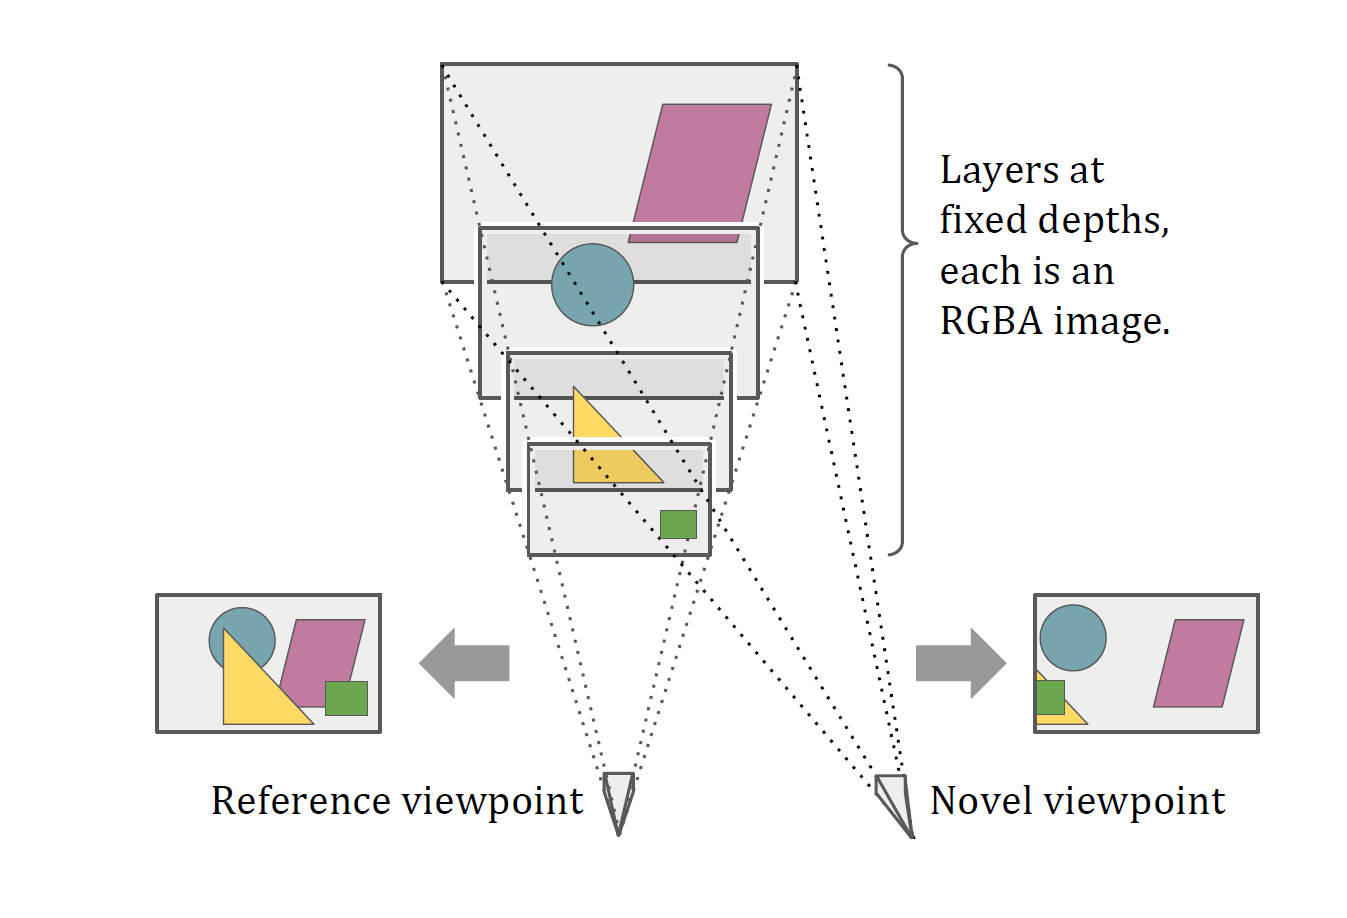
\includegraphics[width=1\columnwidth]{figures/mpi-layered-representation.png}
    \caption{Fronto-parallel planes in MPI layered representation}
    \label{fig:mpi-layered-representation}
\end{figure}
Fig 3. Example of fronto-parallel planes

However, in fact, the coordinates of picture dots cannot be determined with arbitrarily high precision. Rather than that, other sources of noise, such as geometric noise caused by lens distortion or interest point recognition mistake, cause inconsistencies in the picture coordinates that are measured. As a result, the lines created by the associated picture points do not always meet in three-dimensional space. The objective is then to identify a three-dimensional point that fits the observed picture points optimally. Numerous approaches exist in the literature for how to define optimality and how to determine the optimal 3D location. Due to the fact that the various approaches are based on distinct optimality criteria, they generate significantly varied estimations of the 3D point x when noise is present.

tringulation slides on onedrive for diagram
https://en.wikipedia.org/wiki/Triangulation_(computer_vision)
https://www.sciencedirect.com/topics/engineering/disparity-map
https://en.wikipedia.org/wiki/Binocular_disparity
single view or monocular

\chapter{Methods}\label{ch3:methods}

The objective of this work has been to freely rerender concurrent one-on-one video chat frames from the points of view of both participants bidirectionally and in real-time. This would help simulate the experience of conversing face-to-face with a person in the real world. We adopted Tucker and Snavely's~\cite{single_view_mpi} single-view MPI network, for it is the first state-of-the-art open-source single-view view synthesis network, and its popularity is eminent among various organizations since its release in 2020. When we initially ran the publicly available inference part of the network on a video chat frame, we found that the generated disparity map (Equation~\ref{eq:disparity-map}) was visually inaccurate. Comparatively (Figure~\ref{fig:great-off-kilter-disparity}), the inferred disparity map would be much more visually accurate whenever a real estate video frame was processed. The latter outcome is to be expected because Tucker and Snavely's model was originally trained on RealEstate10K~\cite{zhou2018stereo} video dataset. Specifically, certain aspects of the synthesized views, such as image sharpness, would be brilliant for the real estate category of video frames by virtue of the model having been efficiently tweaked and extensively trained by the authors (given contemporary hardware limitations). Yet, synthesized video-chat-related frames alone would seem unnaturally concave/convex at arbitrary positions within each rerendered frame, not to mention the loss of perspectivity and the induction of random distortions occurring within the frame as well.

\begin{figure}[!h]
    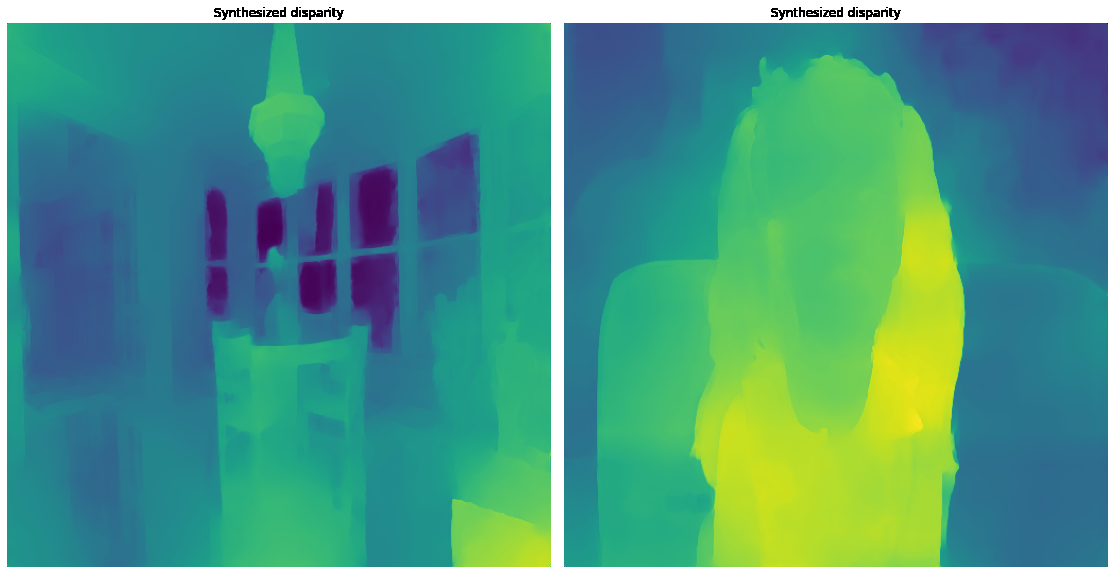
\includegraphics[width=1\columnwidth]{figures/great-off-kilter-disparity.png}
    \caption{Disparity Heat Maps Synthesized by Tucker and Snavely's model~\cite{single_view_mpi} for Real Estate and Video Chat Frames}
    \label{fig:great-off-kilter-disparity}
    {\small The disparity map on the left encodes a real estate scene and the one on the right, a video chat scene. The real estate map successfully shows appropriate heat/depth gradations from the hottest/closest armrest region on the bottom right to the coldest window regions toward the back of the scene. The video chat map, on the other hand, counterintuitively shows that the face of the girl in the scene is situated behind the body, and the couch in it is somehow disjointed.}  
\end{figure}

\section{Approach}\label{sec:approach} 

As a primary step (Figure~\ref{fig:mpi-training-pipeline}), we attempted to increase Tucker and Snavely's depth prediction accuracy for video-chat-relevant frames containing close-up shots of people, so we may see a drastic reduction in the number of artifacts induced in synthesized frames. This involved curating and utilizing both RealEstate10K and MannequinChallenge~\cite{li2019learning} datasets. The latter contains video frames that resemble video chat scenes, as it is composed solely of scenes of people pretending to be mannequins while a camera moves around them, flowing seamlessly from scene to scene. Essentially, we performed transfer learning~\cite{radhakrishnan_what_2019} with the pretrained weights of Tucker and Snavely's model by \textit{fine-tuning}/\textit{refitting} them to a dataset other than the one they were originally trained on. Secondly (Figure~\ref{fig:3d-video-chat-rendering-pipeline}), we introduced the head pose detection submodule of OpenFace 2.2~\cite{baltrusaitis_openface_2018} into the inference pipeline of Tucker and Snavely, so that ``\textit{viewee}" video frames may be rerendered at the head pose obtained from ``\textit{viewer}" frames. We considered a few state-of-the-art open-source head pose estimation models, including WHENet~\cite{zhou_whenet_2020} for its speed and consistency, and ultimately chose OpenFace 2.2 because it works well with the Deep Learning (DL) framework used by Tucker and Snavely (TensorFlow 2.2) and can be installed in the same dockerized environment as COLMAP~\cite{schoenberger2016sfm,schoenberger2016mvs} and the rest of the dependencies needed by our comprehensive pipeline. 

\begin{figure}[!h]
    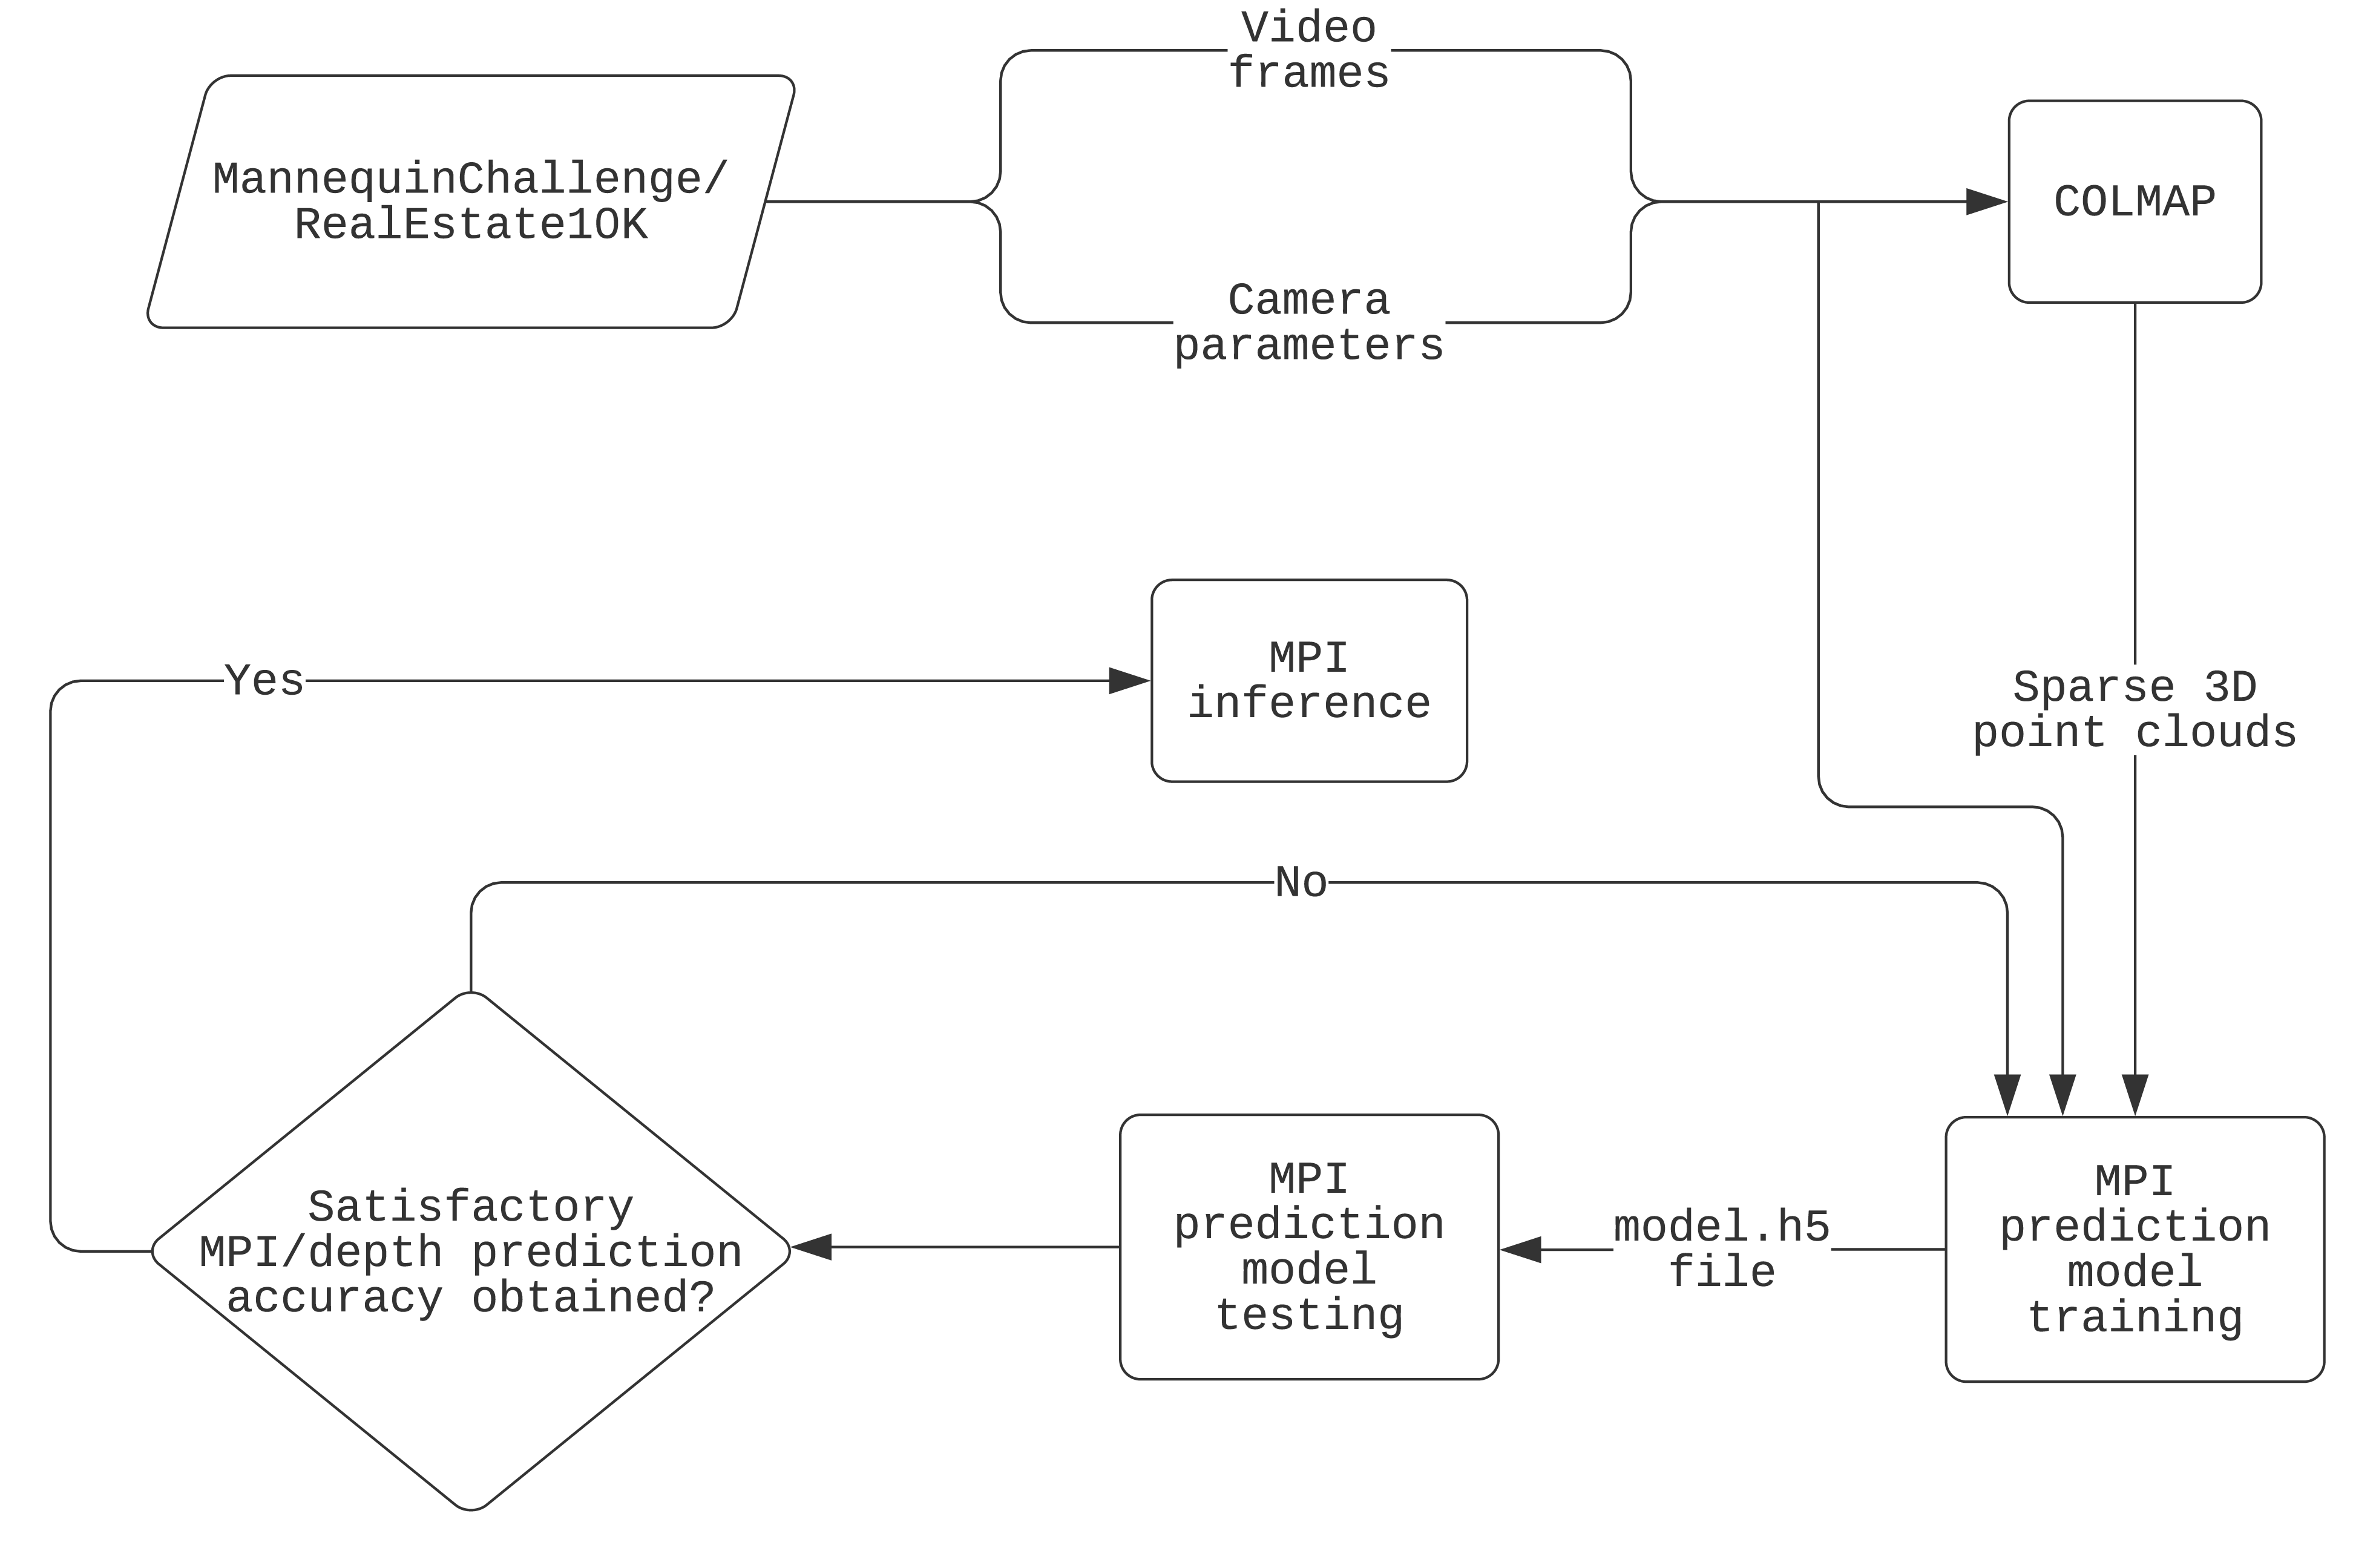
\includegraphics[width=1\columnwidth]{figures/mpi-training-pipeline.png}
    \caption{MPI Training Pipeline}
    \label{fig:mpi-training-pipeline}
\end{figure}

Out of the non-exhaustive set of network components made publicly available by Tucker and Snavely~\cite{single_view_mpi}, a comprehensive inference pipeline on Google Colaboratory (Section~\ref{sec:code-sources}) was one. It greatly helped us with our OpenFace integration and gave us the ability to visualize and present our results and demos in chapter~\ref{ch4:experiments-results} and everywhere else. They couldn't reveal certain other aspects of their codebase due to their proprietary natures. This prompted us to go about recreating Tucker and Snavely's DispNet-like model~\cite{mayer_large_2016} first before retraining it on requisite datasets and repurposing it for video chat view synthesis. We recreated parts of the model from the code released (Section~\ref{sec:code-sources}) by the authors involving their network definition (convolutional layers, kernel sizes, etc.), and the code used by them for rendering views from new camera positions with homographies and related operations (Equation~\ref{eq:rerendered-target}). We then put together other aspects of the network that called for a more involved recreation process like the data loader part and the loss functions (Equation~\ref{eq:aggregate-loss}). Requisite components of input data, including point clouds, had to be extracted and loaded in. One of the key features of Tucker and Snavely is to use sparse point cloud data to make the view synthesis loss scale-invariant (Subsection~\ref{subsec:base-papers}). To obtain such inputs, we processed both datasets with COLMAP and wrote a custom data loader. We took inspiration from Zhou et al.'s~\cite{zhou2018stereo} stereo MPI paper for building the data loader, for the code they tailored to load in data (Section~\ref{sec:code-sources}) was refactored and reused by Tucker and Snavely as well. Their implementations of subsequence selection and random cropping proved useful.

\begin{figure}[!h]
    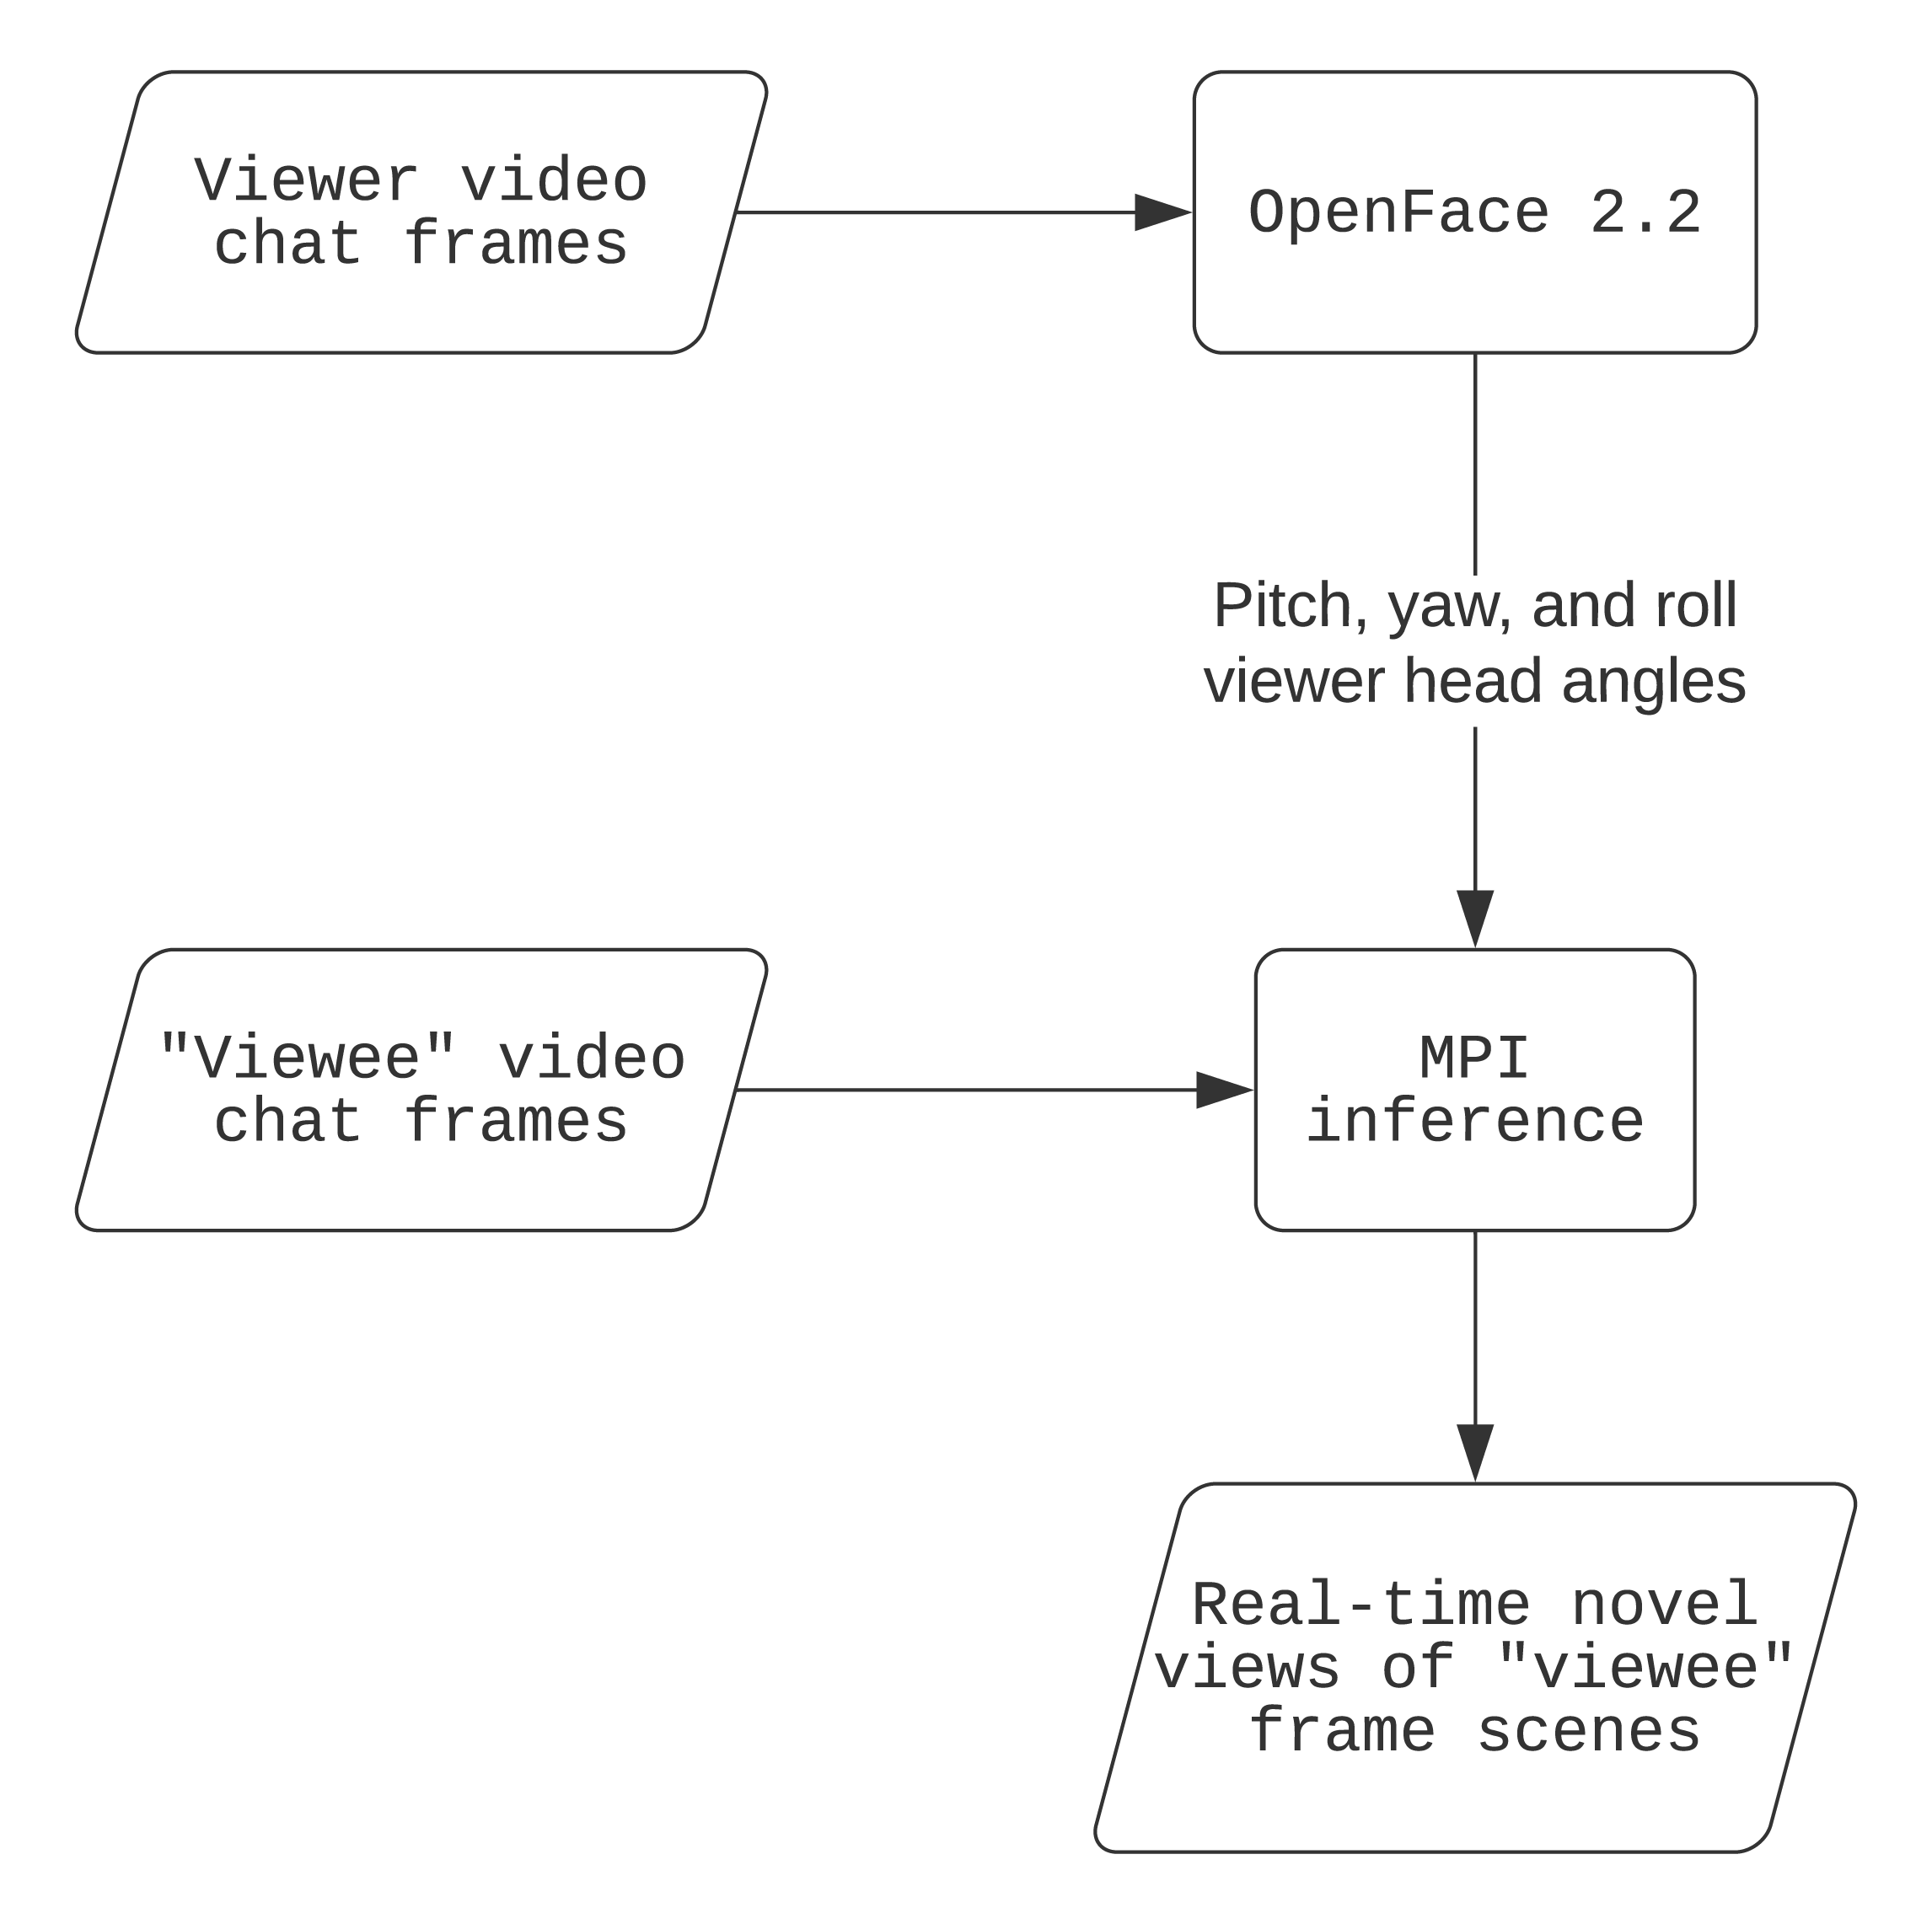
\includegraphics[width=0.60\columnwidth]{figures/3d-video-chat-rendering-pipeline.png}
    \caption{3D Video Chat Rendering Pipeline}
    \label{fig:3d-video-chat-rendering-pipeline}
\end{figure}

We retrained the recreated network in two different ways. One group of model variants was fine-tuned exclusively on the video-chat-relevant MannequinChallenge video dataset~\cite{li2019learning} which is $\sim$96\% smaller than RealEstate10K in training data, as of this writing. The other set of variants was retrained on a combination of both datasets by having the model pick same-sized batches of training data (Subsection~\ref{subsec:base-papers}) randomly and alternatingly from both datasets. We considered addressing this inherent data imbalance problem by making the model pick an appropriate proportion of RealEstate10K frames for every MannequinChallenge frame randomly selected, but ultimately voted against it in favor of resolving more pressing issues such as the training errors mentioned in section~\ref{sec:implementation}. We are grateful to the authors of Tucker and Snavely for forewarning us that there is a risk of overfitting to the much smaller MannequinChallenge dataset, even though it was generally mentioned in both Zhou et al. and Tucker and Snavely that the stereo and single-view models were considerably generalizable to domains besides real estate footage. Hence, we felt the need for deploying the second set of variants to help access this risk. We could also have taken another transfer learning route of freezing all but the last few layers of the model to possibly reduce overfitting but we chose to unfreeze all layers in favor of making the variants wholly robust. The layers were thus free to learn and evolve based on the MannequinChallenge data they were newly exposed to. We stack up these variants to each other and also to the pretrained single-view model and compare their performances in chapter~\ref{ch4:experiments-results}. Finally, after introducing the head pose estimation API of OpenFace 2.2 into the inference pipeline of the variants, we converted estimated head orientations into a form amenable to rendering with MPIs. This involved manipulating yaw, pitch, and roll head angles and the MPI helper functions provided by Tucker and Snavely went a long way in making this possible as well. We also visually verified for if the rerendered frames were getting seemingly aligned with the extracted head poses or not.

\section{Data}\label{sec:data} 

Both Mannequin Challenge~\cite{li2019learning} and RealEstate10K~\cite{zhou2018stereo} datasets were created by roughly the same group of researchers hailing from Google. They involved the same ORB-SLAM2, COLMAP, and scale-normalization procedures of Zhou et al.~\cite{zhou2018stereo} (Subsection~\ref{subsec:base-papers}). Hence, both datasets consist of the same kind of metadata in text files pertaining to the downloadable videos. Each text file begins with the video’s YouTube link on the first line and continues with the details of each COLMAP-processed video frame from the second line onward. Frame details include the timestamp (in microseconds), camera intrinsics, and camera extrinsics. As mentioned in subsection~\ref{subsec:base-papers}, COLMAP is a 3D scene reconstruction pipeline. It attempts to recover the 3D scene structure from even those unstructured 2D images of the scene that do not come tagged with any prior knowledge of camera intrinsics, extrinsics, and nature of objects captured. The extracted scene structure is either in the form of sparse 3D points along with the camera parameters for each input 2D image or in the form of dense 3D points with associated color information. COLMAP's pipeline can be given by: feature detection $\rightarrow$ pairwise feature matching  $\rightarrow$ correspondence estimation $\rightarrow$ incremental structure from motion (Figure~\ref{fig:colmap-photogrammetry-pipeline}). Fortunately, absolute camera poses are not required by the model; only the relative ones made available with the help of COLMAP in these text files are. Our scripts to download and curate all these videos were facilitated by our compilation of a comprehensive Docker container ensuring robustness in code reusability and transferability. Resolving version compatibility issues among our project dependencies such as COLMAP and OpenFace 2.2, both in the Docker container and in Google Colaboratory proved paramount to the successful running of our experiments. All our scripts, notebooks, sample renderings, demos, and most other aspects of our code for this project can be found in our GitHub repository (Section~\ref{sec:code-sources}).

\begin{figure}[!h]
    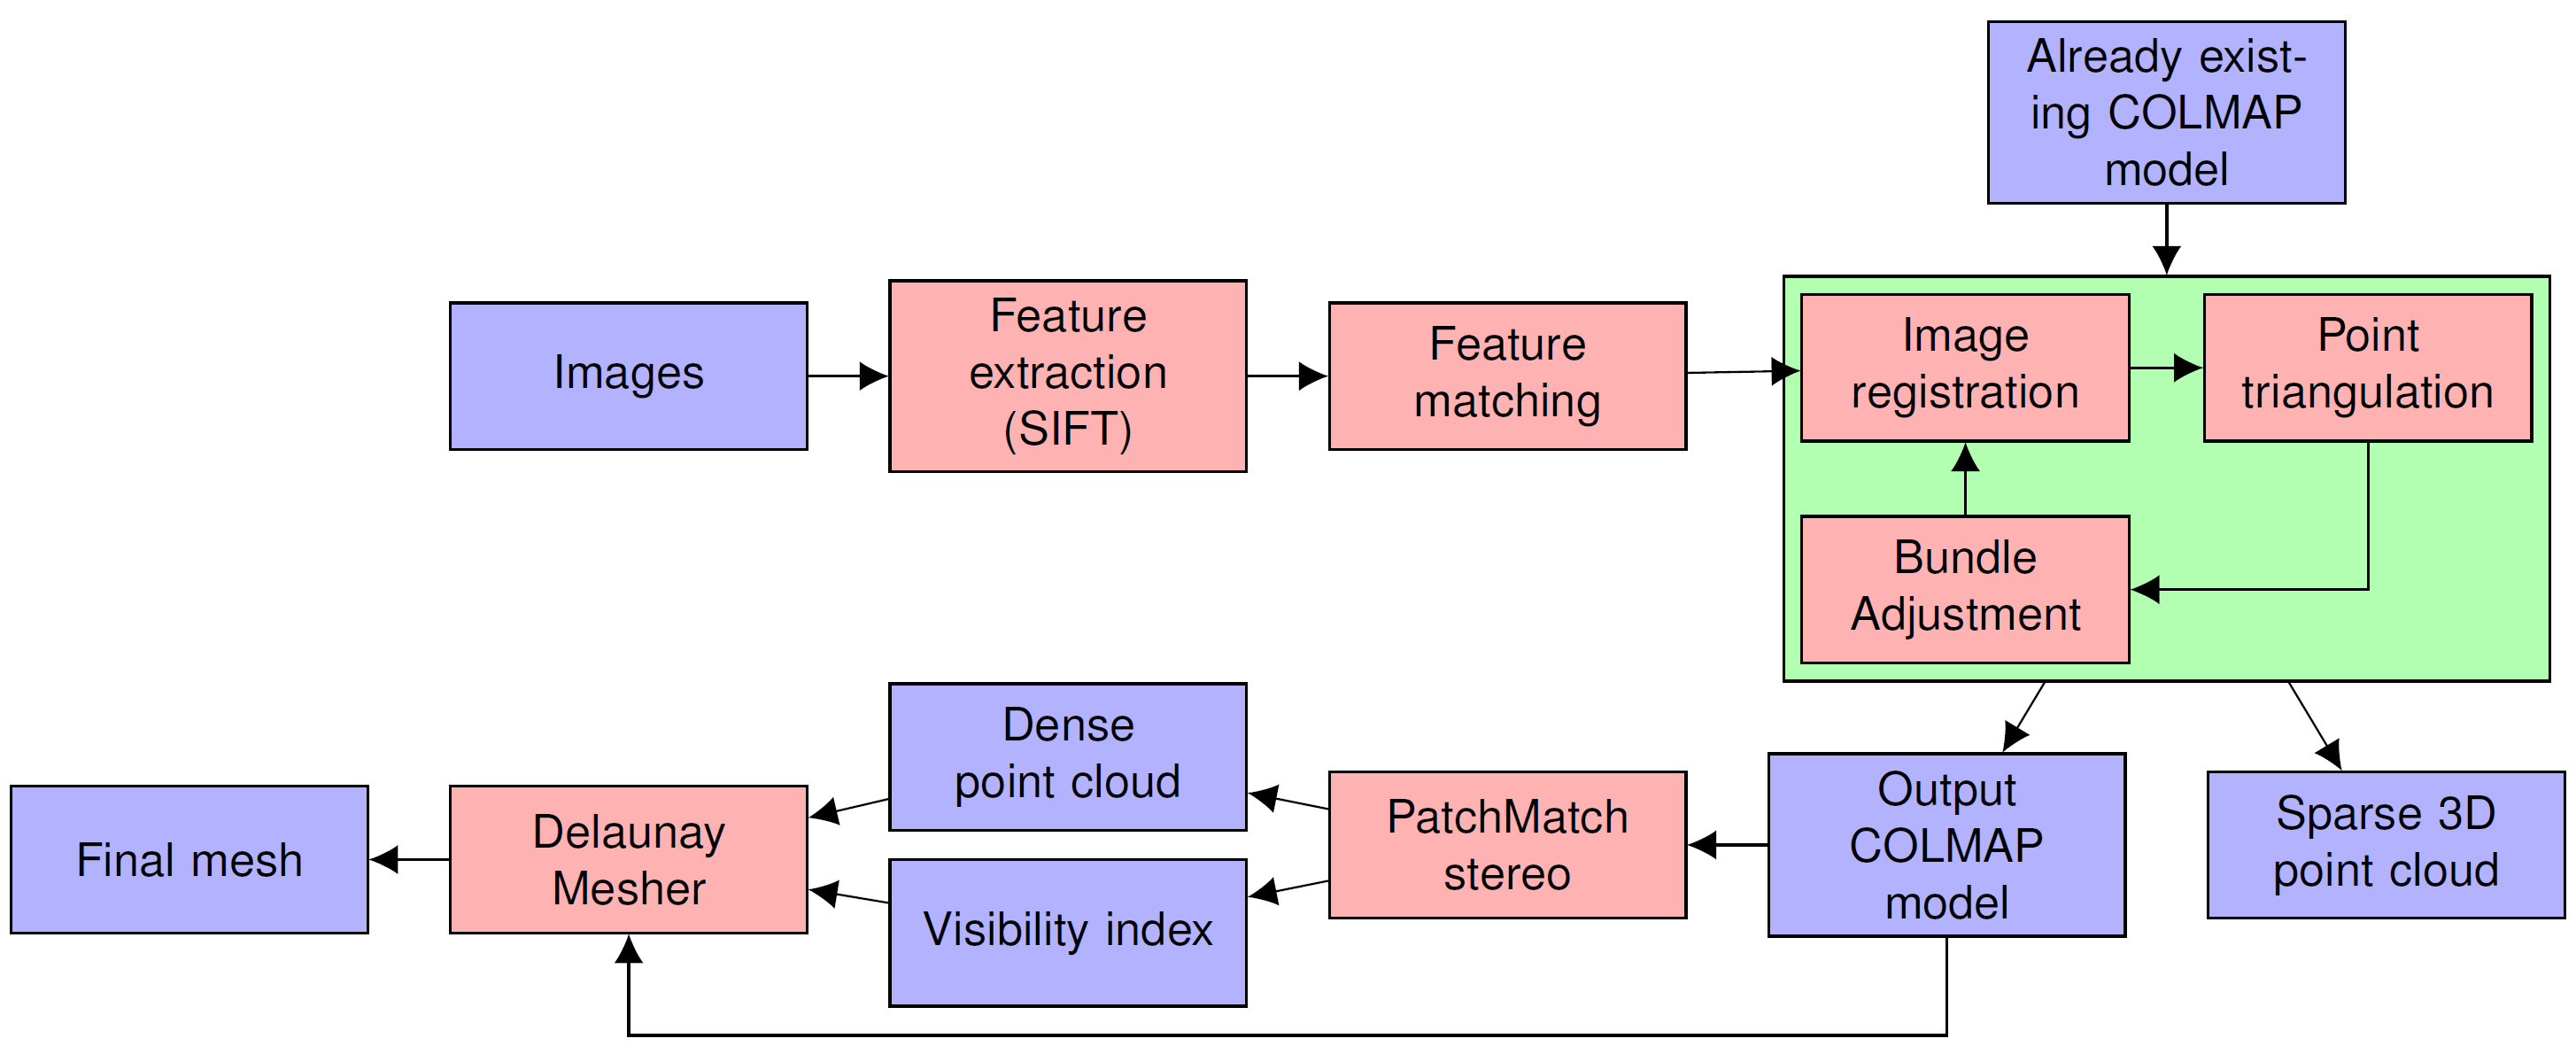
\includegraphics[width=1\columnwidth]{figures/colmap-photogrammetry-pipeline.png}
    \caption{Photogrammetry workflow used in COLMAP~\cite{pinard_does_2021}}
    \label{fig:colmap-photogrammetry-pipeline}
\end{figure}
    
Although our training and testing scripts are designed to crop all incoming video frames to 512$\times$512 pixels, we ensured that we downloaded all videos with youtube-dl at 720p resolution. This uniformity was so we could reduce the number of sources of arbitrariness in the initial process of replicating Tucker and Snavely's~\cite{single_view_mpi} work. Linking youtube-dl with the download management utility aria2~\cite{noauthor_aria2_2021} proved very useful in bolstering youtube-dl’s download speed by optimizing resource utilization. We then targeted addressing youtube-dl download errors. There would inevitably be several partial and/or skipped downloads for various reasons ranging from the videos being taken down from YouTube over time to fixable errors intrinsic to youtube-dl. Moreover, some videos were unavailable in their 720p versions and were discarded by us with the aim of maintaining consistency. In favor of maintaining the pristine versions we chose not to manually convert the varying resolutions to 720p. Although differently scaled videos should theoretically not pose any problem to training or to 3D point cloud generation with COLMAP, we opted again to go with uniformity and consequent ease of reproducibility for one and all.
    
We were finally able to procure 66,861 RealEstate10K videos with 9,095,528 frames and 2,364 MannequinChallenge videos with 117,811 frames, for processing. But not all downloaded videos could be processed. For instance, only $\sim$60000 RealEstate10K videos were actually COLMAP-processed and used for training. This is because the rest of the videos did not meet COLMAP processing requirements. And, it would have taken 200 days to process all 66,861 videos with COLMAP with CPUs alone. Fortunately, we were able to avail the benefits NVIDIA Tesla V100 GPUs (rated the best server models in 2020) at Cal Poly and could bring down the processing time to 25 days. In these ways, we obtained the required points clouds and frames for both training and testing.
















\section{Implementation}\label{sec:implementation} 

We attempted to generate accurate MPI representations for close-up targets such as heads and upper bodies, and improve the pixel accuracies of views synthesized from these MPIs. After putting together the data loader to feed the datasets and point clouds into the network, we recreated loss functions from the textual descriptions in the single-view MPI paper. As mentioned in subsection~\ref{subsec:base-papers}, we likened our training process to Tucker and Snavely~\cite{single_view_mpi} with regard to various aspects such as the use of TensorFlow 2.2, ADAM solver, a pixel loss weight of 1, a smoothness loss weight of 0.5, etc. We experimented with choices of learning rate and depth loss weight but generally picked 0.00001 and 1, respectively, contrary to the 0.0001 and 0.1 used in Tucker and Snavely. We reduced the learning rate because we were fine-tuning the pretrained model rather than training from scratch. The requirement that we had to have view synthesis quality as supervision was fulfilled by taking a frame one frame apart from each chosen training frame as target ground truth. We trained for a number of steps rather than for a number of epochs. Our data loader randomizes batch picking not only for testing but also for training. Moreover, we have not yet been able to go beyond the model experimentation stage. Exposing the model to a wide variety of frames is the way to go in this stage. For the model to be training sequentially on all frames clip by clip, and covering entire datasets multiple times in multiple epochs, it should be free of any errors that impede its progress toward convergence. We have not been able to bring our model up to that stage yet. 

We used wandb.ai~\cite{wandb} for experiment tracking and it proved to be a valuable tool for our entire process. It helped us spin different variants of the model, chiefly characterized by their being trained either on MannequinChallenge alone or on a combination of both datasets. As with some notable attempts at model training in the community, we encountered Not a Number (NaN) gradient errors that took a good chunk of our resolution efforts in this work, but ultimately could not be resolved. NaN losses signal that the issue of vanishing/exploding gradients may be present. In this work, NaN gradients could only be reduced in their frequency of occurrence from once in several hundred steps to once in several thousand steps. wandb.ai helped immensely in resuming not just the training runs themselves but also the activity of logging training metrics right from the point where the run broke off due to a NaN error. What also helped bring down the frequency of encountering NaNs, we believe, was the fact that we removed all those videos from the training/testing process that had at least one frame with a point cloud composed of less than two 3D points. Our Linux command to locate such point cloud \texttt{.txt} files (Section~\ref{sec:code-snippets}) would take about 3 hours to sift through a set of 2500 point cloud directories with one \texttt{.txt} file per video frame. Replacing \texttt{cumprod} used in several places in the single-view MPI source code with \texttt{safe\_cumprod}, as suggested to us by one of the authors of the single-view paper, also helped reduce the frequency of encountering NaNs. One of the issues that we were able to completely resolve was the occasional throwing of \texttt{ValueErrors} by our data loader. We also attempted to redress the rendered artifacts mentioned in section~\ref{sec:approach} and determine if real-time, high-quality view synthesis was indeed possible without game engines.

We used customized training loops with TensorFlow's \texttt{tf.GradientTape} context~\cite{noauthor_custom_nodate}. However, we found that the gradient calculation (Section~\ref{sec:code-snippets}) would take about one minute! We were using a batch size of 8 at that time on an NVIDIA V100 GPU. But the authors of the single-view MPI paper informed us that their gradient calculation would take less than a second even on a single worker. They then correctly diagnosed our issue to be that we were doing everything in \textit{eager mode}, which would lead to the accumulation of a lot of overhead. They suggested that using Keras's \texttt{model.fit}, or using the old estimator system of TensorFlow, or just wrapping things in \texttt{tf.function} should allow the critical parts to run in graph mode and be faster. They also suggested that things were probably too big to fit on our GPU. The authors had used a batch size of 4. We ultimately adopted the use of \texttt{tf.function} wrapper as well as a batch size of 4 and were able to complete implementing our training and testing pipelines.

\begin{figure}[!h]
    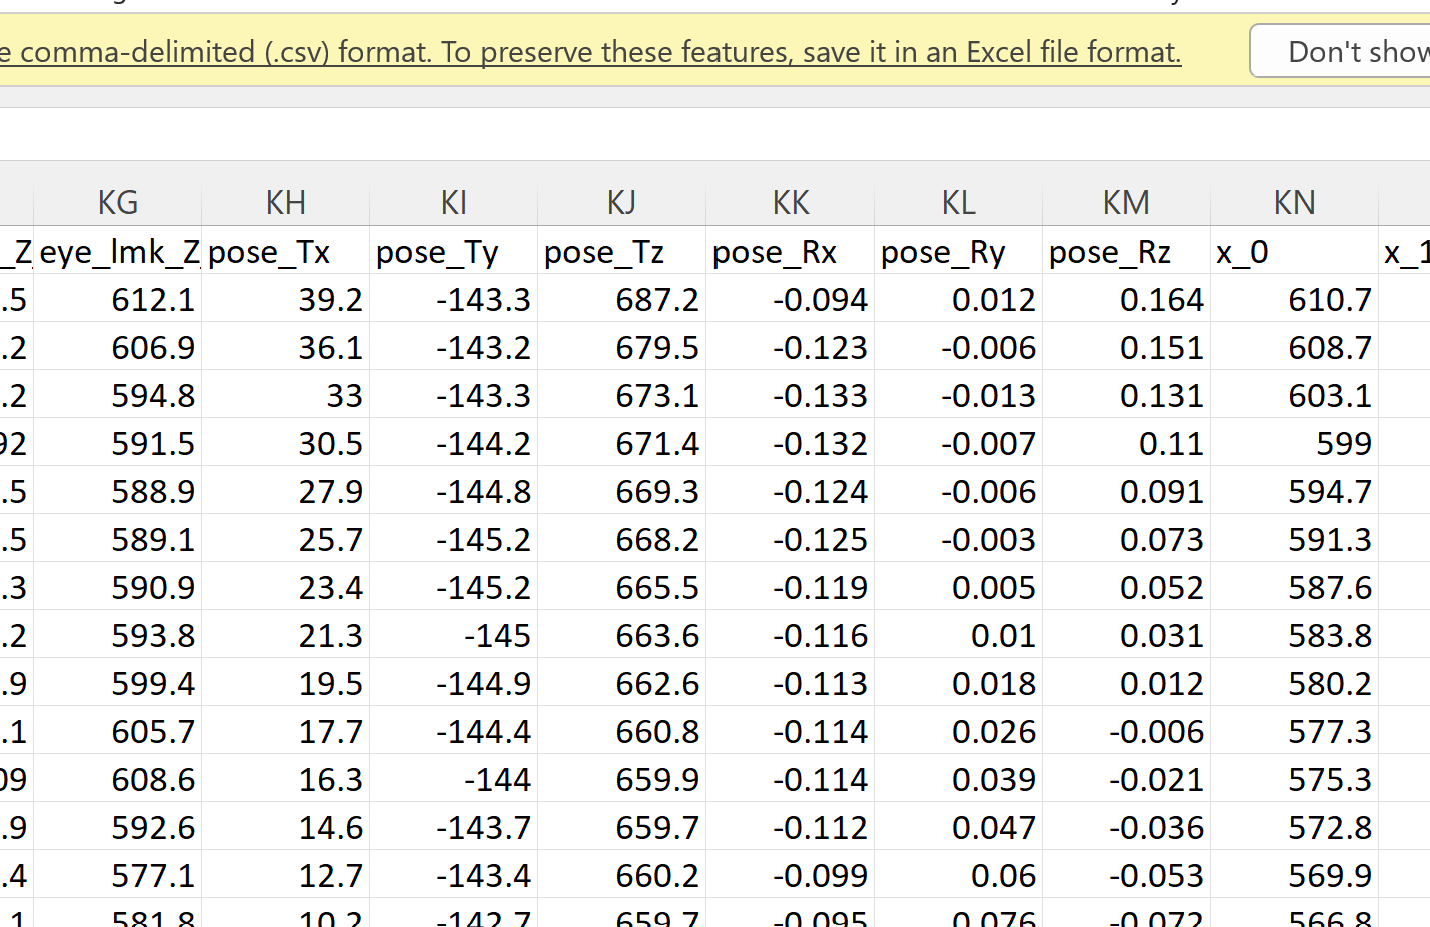
\includegraphics[width=0.75\columnwidth]{figures/openface-csv.png}
    \caption{A Snapshot of OpenFace 2.2~\cite{baltrusaitis_openface_2018} Outputs}
    \label{fig:openface-outputs}
\end{figure}

We then inserted OpenFace 2.2~\cite{baltrusaitis_openface_2018} into the inference pipeline of one of our better performing model variants and attempted to emulate a video chat system, one half at a time. We subjected a ``viewer" video sequence to head pose extraction by OpenFace 2.2 from all frames, as show in figure~\ref{fig:3d-video-chat-rendering-pipeline}. We used one of the utility functions in the single-view MPI modules to extract the yaw, pitch, and roll angles of the ``viewer" frames in a manner conducive to being accepted by the MPI inference. We then rendered the ``viewee" video sequence at the head pose of the ``viewer" frames with matching timestamps. Perhaps more precision could have been added by using not just head pose estimation but also gaze estimation with OpenFace. A snapshot of OpenFace 2.2 outputs for multiple frames in a sequence is shown in figure~\ref{fig:openface-outputs}



% \chapter{Experiments and Results}\label{ch4:experiments-results}

In this chapter, we present some quantitative and qualitative evaluations of the variants of the recreated single-view MPI model retrained on various combinations of MannequinChallenge and RealEstate10K datasets. We use the pretrained weights of the single-view MPI model as the benchmark and compare the abilities of all model variants at hand to generate novel views. We adopt some of the quantitative metrics from Tucker and Snavely's single-view MPI paper~\cite{single_view_mpi} --- PSNR, SSMI~\cite{wang_image_2004}, and LPIPS~\cite{zhang_unreasonable_2018} --- to give numeric values to the similarities between MPI-rendered video frames and the corresponding ground truth target frames the rendering process attempts to replicate. These metrics are computed over all image pixels at a time during evaluation. We based some of our metrics-evaluation scripts on TensorFlow Official Documentation~\cite{noauthor_tfimagepsnr_nodate,noauthor_tfimagessim_nodate}.

The model variants used to compute the metrics stated above are characterized by the following hyperparameters/metadata:
\begin{itemize}
    \item Depth loss weight, as explained in subsection~\ref{subsec:base-papers}.
    \item The number of disparity map channels specified in the \textit{tf.function} input signature for the bilinear sampling function in our training script (Appendix~\ref{sec:code-sources}),\\\textit{sample\_disparities(disparity,\ points)}, involving the predicted disparity and the input visible points.
    \item The lower bound on the number of visible points required per frame; videos with even one frame having the number of visible points below this threshold would be removed from training.
    \item The choice of datasets used to train on --- MannequinChallenge, RealEstate10K, or both.
    \item Whether multiple GPU workers were engaged or not.
\end{itemize}
Even seemingly innocuous hyperparameter values such as those for the number of disparity map channels specified, we believe, could have easily held sway over training progress. Pitting these variants against each other in the three computed metrics helped us select the best variant to simulate half a video chat with each time.

We manually sifted through the in-built test set of the MannequinChallenge dataset to handpick a set of 333 videos. These ORB-SLAM2-curated sequences had video-chat-relevant features. They mostly had the heads and torsos of people being focused upon rather than having wide shots of entire bodies. It was mostly just one or two people in the frames instead of several. Moreover, although not a strict requirement, the head pose of people in these frames was roughly or even very loosely aligned with the camera. There was hardly anybody in any frame that appeared to be looking directly at the camera, as might be expected in an actual video chat. We put these cherry-picked frames in the \textit{test-yes/} bin. We also curated \textit{test-maybe/} and \textit{test-no/} bins. They consisted of the rest of the MannequinChallenge test set with sequences either having no relevance to typical video chat settings (like there being hardly anyone in the frames) in the case of the \textit{test-no/} directory or falling heavily in the gray areas between \textit{test-yes/} and \textit{test-no/} in the case of the \textit{test-maybe/} folder. We even occasionally interspersed the \textit{test-yes/} and \textit{test-maybe/} bins with videos containing sequences that portrayed people facing diametrically opposite the camera. This was just so that we could really challenge the model variant being tested. Table~\ref{tab:video-classifications} shows the classifications of procured videos.

\newcolumntype{L}{>{\raggedright\arraybackslash}p{0.275\textwidth}}
\newcolumntype{M}{>{\raggedright\arraybackslash}p{0.17\textwidth}}
\newcolumntype{N}{>{\raggedleft\arraybackslash}p{0.12\textwidth}}

\begin{table*}[t]
    \centering
    \begin{tabular}{L|M|N|N}
    \toprule
  
    \textbf{Dataset} & \textbf{Bin} & \textbf{Videos} & \textbf{Frames} \\
    
    \midrule
    
    RealEstate10K & \textit{train/} & 66861 & 9095528 \\

    \cmidrule(lr){1-1} \cmidrule(lr){2-2} \cmidrule(lr){3-3} \cmidrule(lr){4-4}
    
    MannequinChallenge & \textit{train/} & 2364 & 117811 \\
    
    \cmidrule(lr){1-1} \cmidrule(lr){2-2} \cmidrule(lr){3-3} \cmidrule(lr){4-4}
    
    MannequinChallenge & \textit{validation/} & 88 & 5928 \\
    
    \cmidrule(lr){1-1} \cmidrule(lr){2-2} \cmidrule(lr){3-3} \cmidrule(lr){4-4}
    
    MannequinChallenge & \textit{test-yes/} & 333 & 12595 \\
    
    \cmidrule(lr){1-1} \cmidrule(lr){2-2} \cmidrule(lr){3-3} \cmidrule(lr){4-4}
    
    MannequinChallenge & \textit{test-maybe/} & 300 & 12831 \\
    
    \cmidrule(lr){1-1} \cmidrule(lr){2-2} \cmidrule(lr){3-3} \cmidrule(lr){4-4}
    
    MannequinChallenge & \textit{test-no/} & 24 & 728 \\
    
    \bottomrule
    \end{tabular}
    \caption{Classifications of Procured Videos}
    \label{tab:video-classifications}
\end{table*}

Of the various aspects of the code that we modeled from the textual descriptions and relevant code snippets obtained from both the single-view and stereo MPI papers, such as \textit{generator\_wandb.py}, \textit{data\_loader.py}, \textit{train\_wandb.py}, and \textit{test.py}, the scripts relevant to the experiments in this section are \textit{test.py} and \textit{generator\_wandb.py} (Appendix~\ref{sec:code-sources}). For testing, the generator first aggregates all video names from the directory input to it, and for each of these, it picks various \textit{reference\_image} and \textit{target\_image} pairs that are internally 5 frames apart. \textit{reference\_image} is the frame \textit{test.py} uses to infer the MPI representation of the scene from, and \textit{target\_image} is supposedly a view of the same scene from a different angle. The possibility that, when the camera moves from one scene to another in the same video, \textit{reference\_image} may depict a scene different from the one captured by \textit{target\_image} is expected to be extremely low as both datasets have been curated by similar ORB-SLAM2 and COLMAP processes. In such hypothetical cases, \textit{target\_image} will be erroneously rendered by \textit{mpi.render} function as the corresponding \textit{rendered\_image}. Nevertheless, since we take the mean of the computed metrics over hundreds of \textit{test.py} processed \textit{reference\_image}-\textit{target\_image} pairs, we believe the final accuracies of a variant's mean metrics will not be off the mark much and shall still be used to determine a variant’s performance satisfactorily. Each of the three metrics is calculated between \textit{target\_image} and \textit{rendered\_image}, which are situated 5 frames apart along the camera trajectory of the respective clip. We did not repeat the same test process for frames 10 apart, which would just have been done to show\footnote{as in the case of the single-view MPI paper} that the longer the baseline between reference/source and target views, the less the rendered image’s accuracy will be. On the same note, we have also not calculated the metrics internally for all processed \textit{(reference\_image, target\_image)} pairs, which would just have been done to catch the hypothetical anomalies of the complete scene changes within a clip, as mentioned before. 

We also took an interesting little detour in our project when we attempted to parallelize training across multiple GPUs. We believed this would have allowed us to increase the batch size\footnote{currently limited to 4 pairs of reference and target images and their respective camera poses and intrinsics, along with the 3D points of the reference image} and thereby let larger and larger parts of our 60000+ training-ready sequences with associated point clouds be used for learning by our recreated model. This would have assisted the model in better avoiding local minima and maxima. But, since TensorFlow's direct conversion procedure that would let standard single-GPU-utilizing scripts become multi-GPU-faring is as yet still an evolving process requiring careful attention to resource allocation issues among the various replicas of the parallelizable aspects of the model\footnote{such as the dataset generator, the loss functions aggregator, etc.} spread across GPUs, our training got undercut after a good start by a resource exhaustion error at training step 178. Nevertheless, we computed all three metrics for this other model variant retrained on MannequinChallenge data using \textit{tf.distribute.MirroredStrategy}, capable of harnessing the power of multiple GPUs.

The rest of this chapter presents the results of the experiments done with the various model variants and the baseline pretrained model. We then cap it all off by presenting the results of incorporating OpenFace 2.2 into the inference pipeline. As of this writing, our generator is only able to pick random pairs of reference and target frames from the 333 \textit{test-yes/} videos. Sequential pair-picking would avoid possible repetition of selected pairs and allow for an exhaustive coverage of the test set. Given that even the smaller of the two datasets has 100,000+ frames and that we have not been able to resolve the issue of the synthesized disparity maps becoming smudgier and smudgier until they turn completely gray/monochromatic even before any of the variants hit 14,000 training steps, it is not very likely that the model may see the same frame twice. So perhaps, computing evaluation metrics with training data can double in as doing the same with validation data itself, even though we haven't set aside validation data. As for the metrics, an LPIPS value of 0 indicates there is either a perfect match between the images being compared or the images being compared are one and the same. To the contrary, SSIM values of 1 indicate a perfect match. Both these metrics range from 0 to 1. PSNR values, measured in decibels (dB), don't generally have an upper limit but values 20 dB and higher are considered acceptable. In calibrating our implementations of these metrics, when we compared an image with itself, we found the mean LPIPS, SSIM and PSNR values over 300 images to be close to 0, 1, and 30, respectively.

\begin{figure}[!h]
    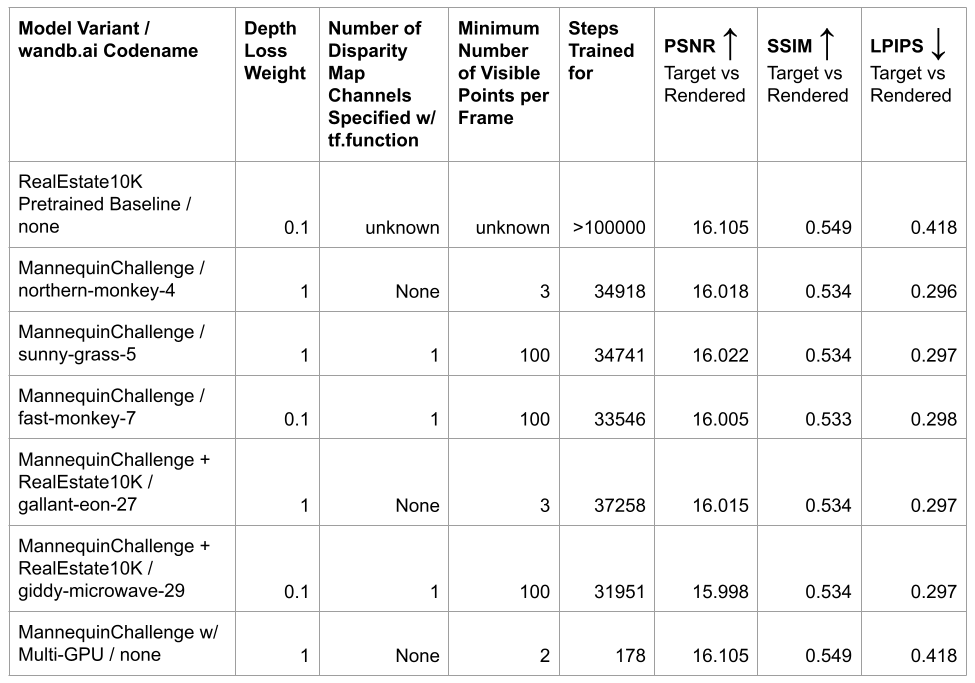
\includegraphics[width=1\columnwidth]{figures/model-variants-metrics.png}
    \caption{Model Variants' Mean PSNR, SSIM, and LPIPS Evaluation Values Over 300 Testing Instances}
    \label{fig:model-variants-metrics}
\end{figure}

We can get a sense of how the variants stack up against one another from figure~\ref{fig:model-variants-metrics}. Perceptual similarity comes the closest to the way humans judge the picture quality of an image. Hence, we chose the variant northern-monkey-4 for the final step of simulating a video chat. These catchy names are automatically allotted by wandb.ai at the start of any training run. If the run is relatively successful, we use the final model produced by it as one of our variants and evaluate its performance. All our variants have been trained to the limit and to the point where the loss becomes less than 1, after having come down all the way from 1188, and stagnates. This has always occurred sooner than 25,000 training steps for all our variants (Figure~\ref{fig:mean-loss}). It goes to show that had we been entirely successful in our implementation of the model, we would also have been able to train for way more than 100,000 steps, similarly to Tucker and Snavely~\cite{single_view_mpi}. Besides, we couldn't really compute the accuracy metric for our models and variants to complement the loss metric as we're training in steps/batches and not epochs.

\begin{figure}[!h]
    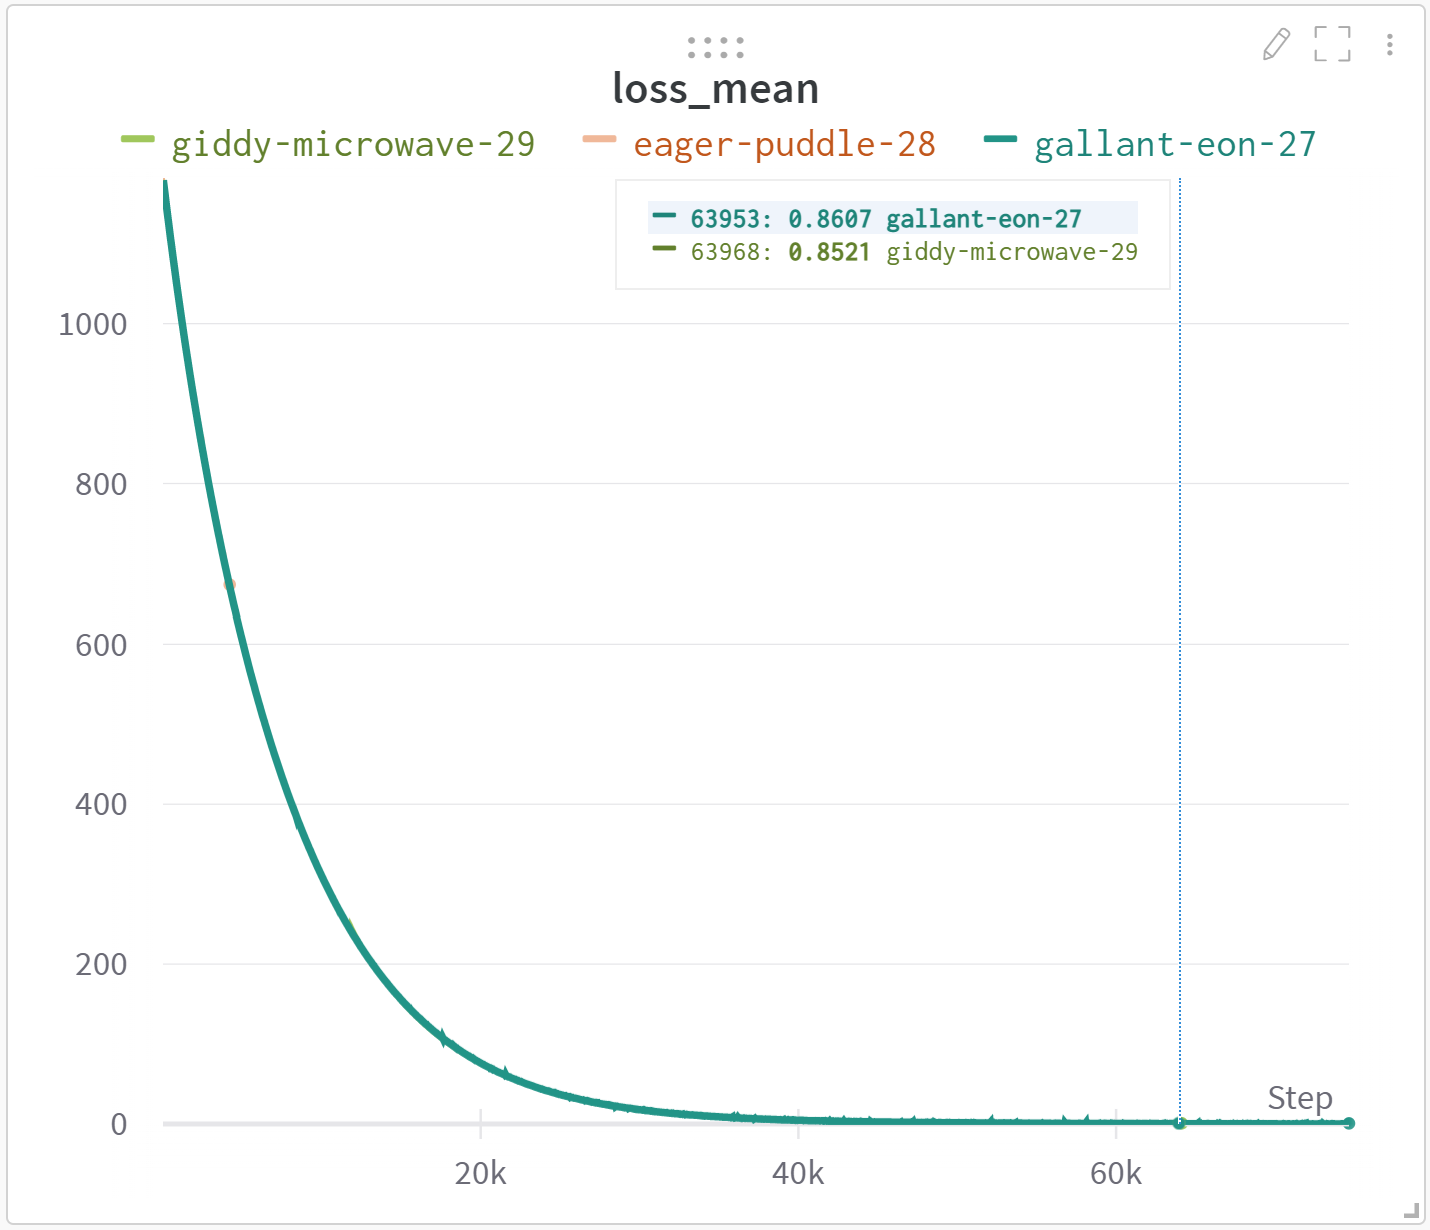
\includegraphics[width=0.75\columnwidth]{figures/mean-loss.png}
    \caption{Typical Mean Loss Chart for Any of Our Training Runs}
    \label{fig:mean-loss}
    {\small wandb.ai somehow always shows twice the number of actual training steps completed on our server. Hence all our variants' training stagnates at 30,000+ steps and not at the 60,000+ steps shown in this wandb.ai-logged loss chart.}
\end{figure}

\begin{figure}[!h]
    \begin{tabular}{cccc}

        \subfloat[]{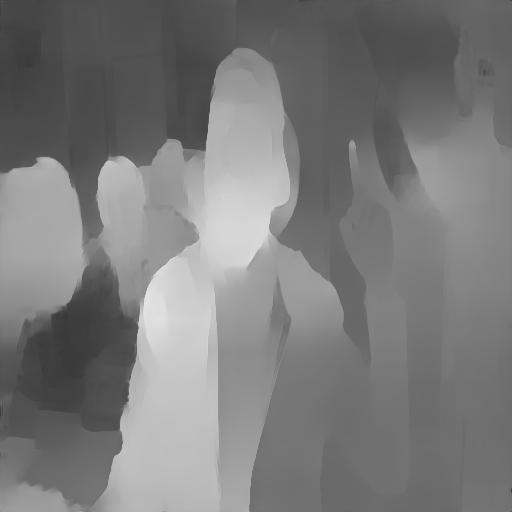
\includegraphics[width = 1.3in]{figures/baseline/000001_image_disparity.png}} &
        \subfloat[PSNR $\uparrow$ Target vs Rendered = 12.345]{\includegraphics[width = 1.3in]{figures/baseline/000001_image_reference.png}} &
        \subfloat[SSIM $\uparrow$ Target vs Rendered = 0.509]{\includegraphics[width = 1.3in]{figures/baseline/000001_image_target.png}} &
        \subfloat[LPIPS $\downarrow$ Target vs Rendered = 0.520]{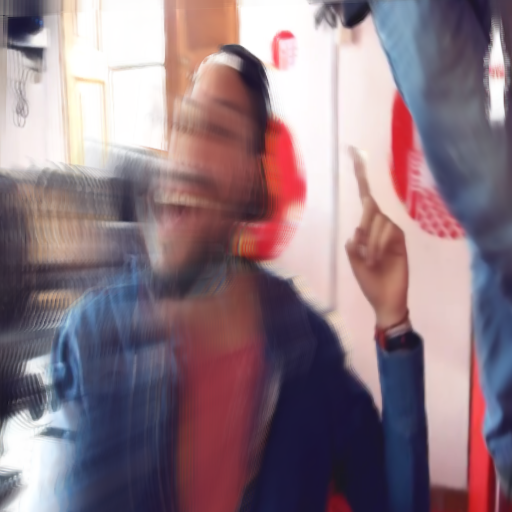
\includegraphics[width = 1.3in]{figures/baseline/000001_image_render.png}}\\
        
        \subfloat[]{
\includegraphics[width = 1.3in]{figures/gallant-eon-27/000001_image_disparity.png}} &
        \subfloat[PSNR $\uparrow$ Target vs Rendered = 12.300]{\includegraphics[width = 1.3in]{figures/gallant-eon-27/000001_image_reference.png}} &
        \subfloat[SSIM $\uparrow$ Target vs Rendered = 0.470]{\includegraphics[width = 1.3in]{figures/gallant-eon-27/000001_image_target.png}} &
        \subfloat[LPIPS $\downarrow$ Target vs Rendered = 0.338]{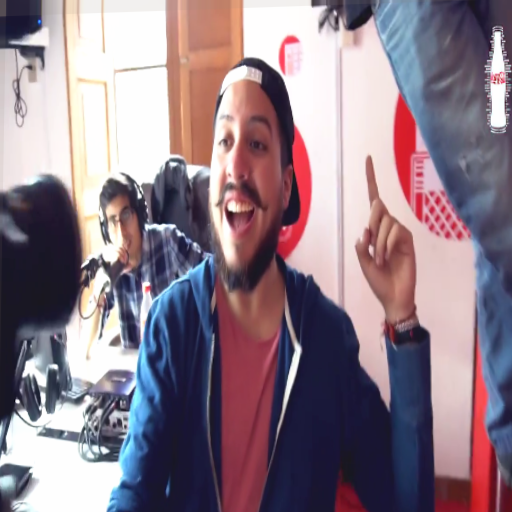
\includegraphics[width = 1.3in]{figures/gallant-eon-27/000001_image_render.png}}\\
        
        \subfloat[]{
\includegraphics[width = 1.3in]{figures/giddy-microwave-29/000001_image_disparity.png}} &
        \subfloat[PSNR $\uparrow$ Target vs Rendered = 12.282]{\includegraphics[width = 1.3in]{figures/giddy-microwave-29/000001_image_reference.png}} &
        \subfloat[SSIM $\uparrow$ Target vs Rendered = 0.470]{\includegraphics[width = 1.3in]{figures/giddy-microwave-29/000001_image_target.png}} &
        \subfloat[LPIPS $\downarrow$ Target vs Rendered = 0.338]{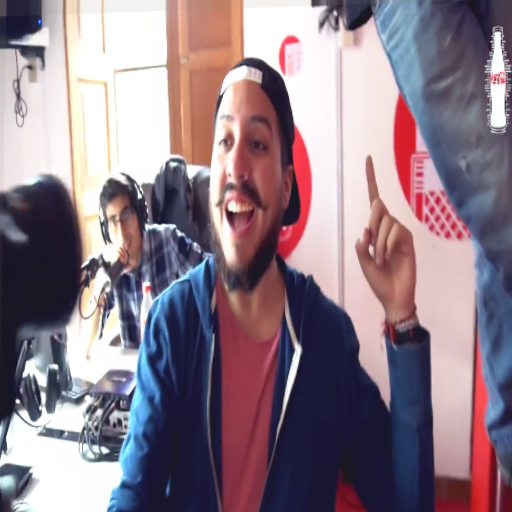
\includegraphics[width = 1.3in]{figures/giddy-microwave-29/000001_image_render.png}}

    \end{tabular}
    \caption{Baseline and (MannequinChallenge+RealEstate10K)-Based Model Variants' Output Visualizations With a MannequinChallenge Target Frame}
    \label{fig:output-visualizations-1}
    {\small Variants from top to bottom: baseline, gallant-eon-27, giddy-microwave-29\\Outputs from left to right: disparity map, reference frame, target frame, rerendered target}
\end{figure}

What further validates our choice of northern-monkey-4 is the set of output visualizations for all relatively successful model variants shown in figures~\ref{fig:output-visualizations-1} and~\ref{fig:output-visualizations-2}. These outputs further reveal that even prior to all our fine-tuning the pretrained model found it hard to synthesize the disparity for video-chat-relevant frames. In the testing example used, the person has clearly moved closer to the camera but the frame synthesized by the baseline model shows ``stack of cards" effects. This could potentially also be the reason that while the picture quality for the renderings seems to have been greatly improved by our fine-tuning (evident from the improved LPIPS values), the already nebulous disparity synthesis (when it comes to video chat frames) has been rendered asunder. It also stands to reason that perhaps depth/disparity is taken more into account by the SSIM metric than the other two metrics, owing to the stark decrease in SSIM values for the fine-tuned variants. It is structural similarity after all, and we have already established that depth is part of the 3D structure of the scene. Hence, we have also been further validated in our efforts to even stick to the course of retraining the baseline model in the first place.

\begin{figure}[!h]
    \begin{tabular}{cccc}

        \subfloat[]{
\includegraphics[width = 1.3in]{figures/northern-monkey-4/000001_image_disparity.png}} &
        \subfloat[PSNR $\uparrow$ Target vs Rendered = 12.315]{\includegraphics[width = 1.3in]{figures/northern-monkey-4/000001_image_reference.png}} &
        \subfloat[SSIM $\uparrow$ Target vs Rendered = 0.470]{\includegraphics[width = 1.3in]{figures/northern-monkey-4/000001_image_target.png}} &
        \subfloat[LPIPS $\downarrow$ Target vs Rendered = 0.337]{\includegraphics[width = 1.3in]{figures/northern-monkey-4/000001_image_render.png}}\\
        
        \subfloat[]{
\includegraphics[width = 1.3in]{figures/sunny-grass-5/000001_image_disparity.png}} &
        \subfloat[PSNR $\uparrow$ Target vs Rendered = 12.315]{\includegraphics[width = 1.3in]{figures/sunny-grass-5/000001_image_reference.png}} &
        \subfloat[SSIM $\uparrow$ Target vs Rendered = 0.470]{\includegraphics[width = 1.3in]{figures/sunny-grass-5/000001_image_target.png}} &
        \subfloat[LPIPS $\downarrow$ Target vs Rendered = 0.337]{\includegraphics[width = 1.3in]{figures/sunny-grass-5/000001_image_render.png}}\\
        
        \subfloat[]{
\includegraphics[width = 1.3in]{figures/fast-monkey-7/000001_image_disparity.png}} &
        \subfloat[PSNR $\uparrow$ Target vs Rendered = 12.284]{\includegraphics[width = 1.3in]{figures/fast-monkey-7/000001_image_reference.png}} &
        \subfloat[SSIM $\uparrow$ Target vs Rendered = 0.471]{\includegraphics[width = 1.3in]{figures/fast-monkey-7/000001_image_target.png}} &
        \subfloat[LPIPS $\downarrow$ Target vs Rendered = 0.339]{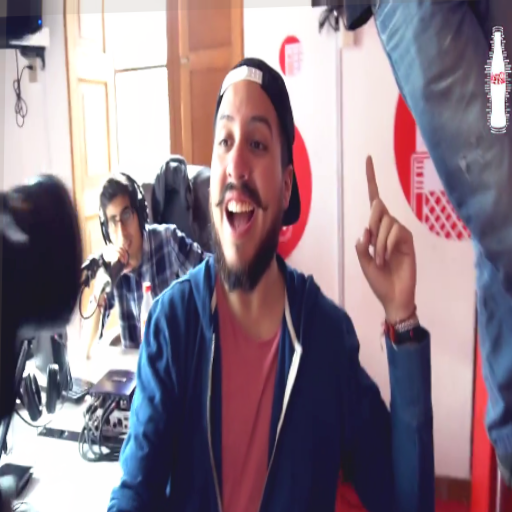
\includegraphics[width = 1.3in]{figures/fast-monkey-7/000001_image_render.png}}\\

    \end{tabular}
    \caption{MannequinChallenge-Based Model Variants' Output Visualizations With a MannequinChallenge Target Frame}
    \label{fig:output-visualizations-2}
    {\small Variants from top to bottom: northern-monkey-4, sunny-grass-5, fast-monkey-7\\Outputs from left to right: disparity map, reference frame, target frame, rerendered target}
\end{figure}

In reference to the qualitative results presented throughout this work, we invoke the reader to adopt Tucker and Snavely's~\cite{single_view_mpi} use of pointers such as the handling of occluded content, the production of undesirable artifacts at the edges of foreground objects, and so on, to qualitatively compare the discrepancies in the results generated by each model variant. Similarly, visually checking for the accuracy of the synthesized disparity maps, as was illustrated at the beginning of chapter~\ref{ch3:methods}, is also useful in verifying the quality of the MPIs produced. We encourage the reader to zoom into the electronic version of this thesis or take to the GitHub repository accompanying this work (Appendix~\ref{sec:code-sources}) for easier visual verification.


% To cap it off with the help of OpenFace 2.2, we also include a few snapshots of how a rerendered frames vary with changes in head pose in figure~\ref{fig:rerendered-with-openface}.  

% As the girl looks to the left the opposite concurrent video frame moves to the right and vice versa
% Please head over to the github repo for this project to observe videos of simultaneous changes simulating a two way video chat.
% testing bring testing to sequential process instead or random using hid generator code

Maybe show and mention the problem with the gradual fading out of disaprity maps for pivotal epochs in the training for the major variants of loki



% \chapter{Discussion}\label{ch:discussion}

% from deep stereo paper the causes for overfitting

% Deep networks have enjoyed huge success in recent
% years, particularly for image understanding tasks [20, 29].
% Despite these successes, relatively little work exists on applying
% deep learning to computer graphics problems and especially
% to generating new views from real imagery. One
% possible reason is the perceived inability of deep networks
% to generate pixels directly, but recent work on denoising
% [35], super-resolution [6], and rendering [21] suggest
% that this is a misconception. Another common objection is
% that deep networks have a huge number of parameters and
% hence are prone to overfitting in the absence of enormous
% quantities of data, but recent work [29] has demonstrated
% state-of-the-art deep networks whose parameters number in
% the low millions, greatly reducing the potential for overfitting.

% from deep stereo on the success of neural nets

% In this work we present a new approach to new view synthesis
% that uses deep networks to regress directly to output
% pixel colors given the posed input images. Our system
% is able to interpolate between views separated by a
% wide baseline and exhibits resilience to traditional failure
% modes, including graceful degradation in the presence of
% scene motion and specularities. We posit this is due to the
% end-to-end nature of the training, and the ability of deep
% networks to learn extremely complex non-linear functions
% of their inputs [25].
% Additionally, although we focus on its application
% to new view problems here, we believe that the
% deep architecture presented can be readily applied to other
% stereo and graphics problems given suitable training data.
% Because
% of the variety of the scenes seen in training our system is robust
% and generalizes to indoor and outdoor imagery, as well
% as to image collections used in prior work.

Through this thesis, we have had the opportunity to simulate both halves of a 2-way pipeline that is able to render novel views from the perspectives of both participants in a video chat. Going by the synthesized monochromatic disparity maps and even by the SSIM values, we found that our model variants struggled to synthesize disparity well. Going by the LPIPS values, we found that they excelled at synthesizing the actual target view itself. This is indeed unexpected owing to the fact that only one of the given 32 MPI layers is able to essentially duplicate the reference image in its entirely.

A further testimony to this improvement can be obtained by inspecting the performance of even the prematurely halted multi-GPU variant. It performs at par with the original pretrained model which indicates that the pretrained model has begun to continue where it left off and specialize in processing video-chat-like frames. It would have run properly if not for the resource errors mentioned in the earlier sections (let's mention the section number here) that could point to underlying issues like possible unchecked growth of TensorFlow graphs per pipeline replica or such. This seems to be the case even though the replicas seem to be getting properly allocated inputs and their respective outputs also seem to be getting well gelled together in the end.

Although the sharpness of the rerendered images is almost twice as good with our chosen model variant as with the pretrained baseline, the predicted MPIs layers have all but collapsed to a single depth layer. This is also evident from the way the training would start to produce completely gray disparity maps from around step 14000 onward, as noted in chapter~\ref{ch4:experiments-results}. We believe that the reason for this is more likely to be found in the weights we assigned to our various loss functions that aggregate into a mean loss. Ablation experiments involving taking out the pixel loss and/or bringing the smoothness loss way down would help to isolate the issue even more. Furthermore, we believe that if we can crack the reason for some model variants' disparity maps turning gray faster than others (Figure~\ref{fig:gray-disparity-maps}), we would be able to nail the root issue with these reconstructed models of ours. Although we made our best efforts to reconstruct the loss functions and the rest of training setup as close to the textual descriptions in the paper as possible, it would definitely shine a lot more light on the root cause of the problem if we are able to access the training script of the authors --- something that they've had to keep from the public. Also, since we were also meticulous with our data curation, we don't believe it is likely that the input data has any part to play in the generation of NaN loss errors.

One of the obvious next steps would be to perform \textit{hyperparameter sweeps} with wandb.ai to find optimal hyperparameters, including the weights of the loss functions, and potentially solve the vanishing/exploding gradients problem which could very well be related to the issue of the swiftly saturating disparity maps. If we are actually able to get the plan to work, it would reveal why the pretrained model found it hard to synthesize disparity for video chat frames in the first place: it was not exactly as generalizable as the authors hinted it might be. But, if after running all possible hyperparameter sweeps with something like wandb.ai, we still find that the model performs poorly, then the obvious next thing to look at would be the actual training scripts used by the authors to discover how way off the mark we could have been in replicating their network.

% \chapter{Conclusion}\label{ch:conclusion}
\section{Conclusion}\label{sec:conclusion}


In this thesis, we have not created novel models or datasets but have rather curated preexisting datasets and retrained a state-of-the-art CNN. Data curation has been an essential part of our work as the datasets' YouTube videos are subject to modifications over time. These modifications are in terms of the videos being taken down from YouTube or the required 1280$\times$720 pixel (720p) resolution versions of them becoming unavailable, etc. The curation process included action items like downloading and training only on 720p versions of the datasets' videos so as to minimize the chances of running into training errors, etc., as explained in section~\ref{sec:data}. As for simulating the 3D video chat experience itself, we linked-up the API of OpenFace 2.2~\cite{baltrusaitis_openface_2018} --- a preexisting head pose estimation model --- to the MPI inference procedure so the MPI inference may generate novel views rendered in the head pose evaluated by OpenFace 2.2, as explained in section~\ref{sec:implementation}.

We used MPI to solve 3D video chat problem because of it real-time view and other view synthesis properties mentioned in the base paper section above. High quality, spatially-consistent, and high-resolution synthesis by rendering with MPIs which are essentially mini-local-light-field representations have been accomplished.
% in defence mention that MPI essentially constructs a mini light field.
\section{Future Work}\label{sec1:future-work}
Maybe we could implement taking the average of the head poses of multipe people in the video frames of video conferences instead of just video chat and make their average head pospe change the scene rendering viepoint of teh secne to be rerenered.

Through this thesis, I had the opportunity to form a 2-way pipeline that is able to render new views from the perspectives of both the participants in Video Chat conversation.

Increase the training speed of the MPI model by making it a multi-GPU model with the constantly-evolving, cutting-edge tf.distribute.Strategy API for distributed training with TensorFlow/Keras.
This would allow for feeding a lot more images/video-frames to the model, which would further reduce the accuracy of the model.

Using Grad-CAM to locate the bottlenecks in the recreated MPI neural net to optimize hyperparameter tuning for producing more accurate results, esp. predicted depths / disparity.
https://www.pyimagesearch.com/2020/03/09/grad-cam-visualize-class-activation-maps-with-keras-tensorflow-and-deep-learning/


Render in both directions, making the pipeline two-way and then proceed to make it realtime by involving a game engine or any other framework capable of realtime rendering. 

Try training on variable resolution video frames and not all just 1280x720 ones

Ideal for a headless server?

make use of docker multistage builds to have all components in a single dockerfile
with multiple froms like tf/tf-gpu-2.2 as well as nvidia-cuda10.2-devel-ubuntu18.04

possible hypothesis: did cuda support improve disparity map

possible hypothesis: cuda gpu support is possibly not required for OpenFace inference

features of OPenFace like head pose estimation may still work without CUDA recognition by the server either COlab or El Capitan 

need gpu support for maybe mpi training alone and not any other components of the pipeline as the rest of the pipeline is just inference

COLMAP will be quicker with GPU
https://colmap.github.io/faq.html#available-functionality-without-gpu-cuda

major hypothesis: one major reason with disparity map to be less because the batch size was only 4 frames at once   
if multi-gpu access were available then disparity map would have been better 

Mainly mpi and maybe even colmap (for inference speed) seem to require GPU/CUDA support. I've been trying to get GPUs to be used by all my packages on Docker like MPI, COLMAP and their dependencies OpenCV, Dlib etc.
I doesn't seem to work yet. So I'll resort to using these packages on Docker without GPU support for now. 

in videos we have recording of my insights today - 8/15/21
been falling behind and didn't report until resukts 

and update to flagship versions

the main thing Dr ventura is that the CUDA install was broken and I needed it for multiple programs like dlib, openface, notwithstanding colmap 

ask prof ventura to update the nvidia drivers 

why did i go off on a tangent?
https://stackoverflow.com/questions/43022843/nvidia-nvml-driver-library-version-mismatch
Available functionality without GPU/CUDA

https://colmap.github.io/faq.html#available-functionality-without-gpu-cuda
If you do not have a CUDA-enabled GPU but some other GPU, you can use all COLMAP functionality except the dense reconstruction part. However, you can use external dense reconstruction software as an alternative, as described in the Tutorial. If you have a GPU with low compute power or you want to execute COLMAP on a machine without an attached display and without CUDA support, you can run all steps on the CPU by specifying the appropriate options (e.g., --SiftExtraction.use_gpu=false for the feature extraction step). But note that this might result in a significant slow-down of the reconstruction pipeline. Please, also note that feature extraction on the CPU can consume excessive RAM for large images in the default settings, which might require manually reducing the maximum image size using --SiftExtraction.max_image_size and/or setting --SiftExtraction.first_octave 0 or by manually limiting the number of threads using --SiftExtraction.num_threads.

nvidia-smi
Failed to initialize NVML: Driver/library version mismatch


what is cuda and nvcc all about?
https://varhowto.com/check-cuda-version/

dockerfile colmap run needs to be explained with video clip in MAnnequinChallenge

proof that gpu is being used by colmap in images in MannequinChallenge


https://linuxize.com/post/linux-time-command/
time all functions

make sure I'm able to restart the model at any poit and continue traning whre I left off and add datasets 

I need info on inference code 

Ask ventura why did yoyu say the disparity was bad

Hopefully successfully able to use the latest versions of all components of the mpi pipeline for both training and inference  

Another application would be if we have a VR headset with a camera on it we can track the rotation of the camera and by doing that you're tracking the rotation of the person's head so that you can render the VR content at the right angle

Ask prof ventura is colmap autmatically redoes all error videos 
Ask pro ventura about copyright for his own epipolar geometry lectures

stereo = 2 images pretty close to each other paired in a special way so that you can get really dense estimations of the depth so basically for every pixel you could get a depth estimate rather than some sparse sampling of keypoints
canonical stereo case only have pure horizontal translation and no rotation and no other translations in Y or Z  

blueer values are closer and redder values are farther away in disparity maps

check 7000 train set and 1400 test set of 2018 paper

why doesn't 2020 and 2018 papers employ SLAM algorithms directly from COLMAP and not indorectly by themsellves or are they refereing to the same slam algorithms

overfitting can be further reduced by using a cnn in the place of a gradient descent algorithm like flynn et all deep stereo 2019 i.e., essentially combining 2020 paper with this predecessor 
chaekc the first chaPpter of interduction of 2019 deep stereo for more info abou this
As a consequence, the network takes much larger strides along the direction of optimization and converges much sooner and with more accuracy than a network using standard gradient descent.

Actually, the DeepView paper has a beautiful software to customized, visualize, and render any type of MPI! It's kind of like the state of the art MPI manipulator.~\url{https://augmentedperception.github.io/deepview/}. So maybe improve the 2020 MPI html visualizer upto the standarsd of the deep view one or atleast use it to tweak and experiment the various MPI paraeters lik number of layers etc before deploying and training and testing.

Adam is better than regular stochastic gradient descent but still not superior to Flynn et al.'s~\cite{flynn_deepview_2019} implementation of learned gradient descent.


\nocite{*}
\bibliography{bibliography}

% Indents Appendix in Table of Contents
\makeatletter
\addtocontents{toc}{\let\protect\l@chapter\protect\l@section}
\makeatother

% Hack to make Appendices to appear in Table of Contents
\addtocontents{toc}{%
   \noindent APPENDICES
}
\begin{appendices}
\begin{appendices}
\chapter{Code Sources and Snippets}\label{app:code-sources-snippets}

\section{Code Sources}\label{sec:code-sources}

\begin{outline}
    \1 Tucker and Snavely's~\cite{single_view_mpi} network definition: \href{https://github.com/google-research/google-research/blob/ea313c6e96acce6c863de41615c6cf4079b8ca94/single_view_mpi/libs/nets.py#L146}{\texttt{nets.mpi\_from\_image}}
    \1 Tucker and Snavely's rendering code: \href{https://github.com/google-research/google-research/blob/ea313c6e96acce6c863de41615c6cf4079b8ca94/single_view_mpi/libs/mpi.py#L232}{\texttt{mpi.render}}
    \1 Zhou et al.'s~\cite{zhou2018stereo} data loader: \href{https://github.com/google/stereo-magnification/blob/f2041f80ed8c340173a6048375ba900201c1f1e7/stereomag/loader.py}{\texttt{loader.py}}; \href{https://github.com/google/stereo-magnification/blob/f2041f80ed8c340173a6048375ba900201c1f1e7/stereomag/datasets.py}{\texttt{datasets.py}}
    \1 The GitHub repository for this thesis: \url{https://github.com/anuraguppuluri/view-synthesis.git}
\end{outline}

\section{Code Snippets}\label{sec:code-snippets}

\begin{outline}
    \1 Gradient calculation:
        \2 \texttt{grads = tf.GradientTape().gradient(loss,}
        \2 \texttt{model.trainable\_weights)}
\end{outline}

\end{appendices}

\end{appendices}

\end{document}
